% Fixing: Too many math alphabets used in version normal
\newcommand\hmmax{0}
\newcommand\bmmax{0}
\documentclass[dvipsnames,conference]{IEEEtran}

\usepackage[T1]{fontenc}
\usepackage[scaled=.83]{beramono}

\usepackage[colorinlistoftodos]{todonotes}
\usepackage[inference]{semantic}
\usepackage[switch]{lineno}
\usepackage{halloweenmath}
\usepackage{fontawesome5}
\usepackage{listofitems}
\usepackage{breakcites}
\usepackage{glossaries}
\usepackage{hyperref}
\usepackage{cleveref}
\usepackage{stmaryrd}
\usepackage{marvosym}
\usepackage{listings}
\usepackage{amssymb}
\usepackage{amsmath}
\usepackage{nameref}
\usepackage{amsthm}
\usepackage{xspace}
\usepackage{xfrac}
\usepackage{tikz}
\usepackage{soul}
\usepackage{bm}

%\renewcommand\UrlFont{\color{blue}\rmfamily}
%\newcommand{\url}[1]{\lstinline{#1}}

\setul{0.95ex}{0.3ex}


\usetikzlibrary{calc,decorations.pathmorphing,shapes,positioning}
\newcounter{sarrow}
\newcommand\xrsquigarrow[1]{%
\stepcounter{sarrow}%
\mathrel{\begin{tikzpicture}[baseline= {( $ (current bounding box.south) + (0,-0.5ex) $ )}]
\node[inner sep=.5ex] (\thesarrow) {$\scriptstyle #1$};
\path[draw,<-,decorate,
  decoration={zigzag,amplitude=0.7pt,segment length=1.2mm,pre=lineto,pre length=4pt}]
    (\thesarrow.south east) -- (\thesarrow.south west);
\end{tikzpicture}}%
}
\makeatletter
\newcommand{\xRightarrow}[2][]{\ext@arrow 0359\Rightarrowfill@{#1}{#2}}
\makeatother

\newcommand{\thmref}[1]{\cref{#1}~(\nameref{#1})}
\newcommand{\Thmref}[1]{\Cref{#1}~(\nameref{#1})}

%%%%
% TODO macros
\newcommand{\MK}[1]{\todo[color=orange!30]{TODO: #1}}
\newcommand{\MKin}[1]{\todo[color=orange!30,inline]{TODO: #1}}
\newcommand{\MP}[1]{\todo[color=blue!30]{TODO: #1}}
\newcommand{\MPin}[1]{\todo[color=blue!30,inline]{TODO: #1}}
\newcommand{\hltt}[1]{\begin{center}\fbox{\color{green}\large{#1}}\end{center}}

% Approx
\newcommand{\pages}[1]{}%\xspace\todo{\textbf{($\sim$#1 pages)}\xspace}}

%%%%
% Colors
\newcommand{\neutcol}[0]{black}
\newcommand{\stlccol}[0]{RoyalBlue}
\newcommand{\irccol}[0]{Apricot}
\newcommand{\ulccol}[0]{RedOrange}
\newcommand{\objcol}[0]{Emerald} %CarnationPink}
\newcommand{\commoncol}[0]{black}

\newcommand{\col}[2]{\ensuremath{{\color{#1}{#2}}}}

\newcommand{\com}[1]{\ensuremath\mathit{\col{\neutcol}{#1}}}
\newcommand{\src}[1]{\ensuremath\mathsf{\col{\stlccol}{#1}}}
\newcommand{\irl}[1]{\ensuremath\mathit{\col{\irccol}{#1}}}
\newcommand{\trg}[1]{\ensuremath\mathbf{\col{\ulccol}{#1}}}
\newcommand{\obj}[1]{\ensuremath\mathtt{\col{\objcol}{#1}}}

%%%%
% Text Decorations
\newcommand\BrText[2]{%
  \par\smallskip
   \noindent\makebox[\textwidth][r]{$\text{\scriptsize #1}\left\{
    \begin{minipage}{\textwidth}
    #2
    \end{minipage}
  \right.\nulldelimiterspace=0pt$}\par\smallskip
}
\newcommand{\mi}[1]{\ensuremath{\mathit{#1}}}
\newcommand{\mr}[1]{\ensuremath{\mathrm{#1}}}
\newcommand{\mt}[1]{\ensuremath{\texttt{#1}}}
\newcommand{\mtt}[1]{\ensuremath{\mathtt{#1}}}
\newcommand{\mf}[1]{\ensuremath{\mathbf{#1}}}
\newcommand{\mk}[1]{\ensuremath{\mathfrak{#1}}}
\newcommand{\mc}[1]{\ensuremath{\mathcal{#1}}}
\newcommand{\ms}[1]{\ensuremath{\mathsf{#1}}}
\newcommand{\mb}[1]{\ensuremath{\mathbb{#1}}}
\newcommand{\msc}[1]{\ensuremath{\mathscr{#1}}}

\newcommand{\bul}[1]{{\setulcolor{RoyalBlue}\ul{#1}}}
\newcommand{\rul}[1]{{\setulcolor{RedOrange}\ul{#1}}}
\newcommand{\iul}[1]{{\setulcolor{Apricot}\ul{#1}}}
\newcommand{\oul}[1]{{\setulcolor{Emerald}\ul{#1}}}
\newcommand{\pul}[1]{{\setulcolor{CarnationPink}\ul{#1}}}

\newcommand{\lock}{\ensuremath\text{\scriptsize\faIcon{lock}}}
\newcommand{\unlock}{\ensuremath\text{\scriptsize\faIcon{lock-open}}}

\newcommand{\tup}[2]{\ensuremath (#1 %
  \readlist\myterms{#2}%
  \foreachitem\x\in\myterms{;\x}%
  )%
}

\newcommand{\isdef}[0]{\ensuremath{\mathrel{\overset{\makebox[0pt]{\mbox{\normalfont\tiny\sffamily def}}}{=}}}}

%%%%
% List of contributions
\newcounter{contrib}
\newcommand{\contribnum}[0]{\stepcounter{contrib}{\arabic{contrib}}.~}
\newcommand{\contribution}[1]{\smallskip\noindent\textbf{{#1.}\xspace}}

%%%%
% A symbol for Coq-verified theorems.
\newcommand{\BareCoqSymbol}{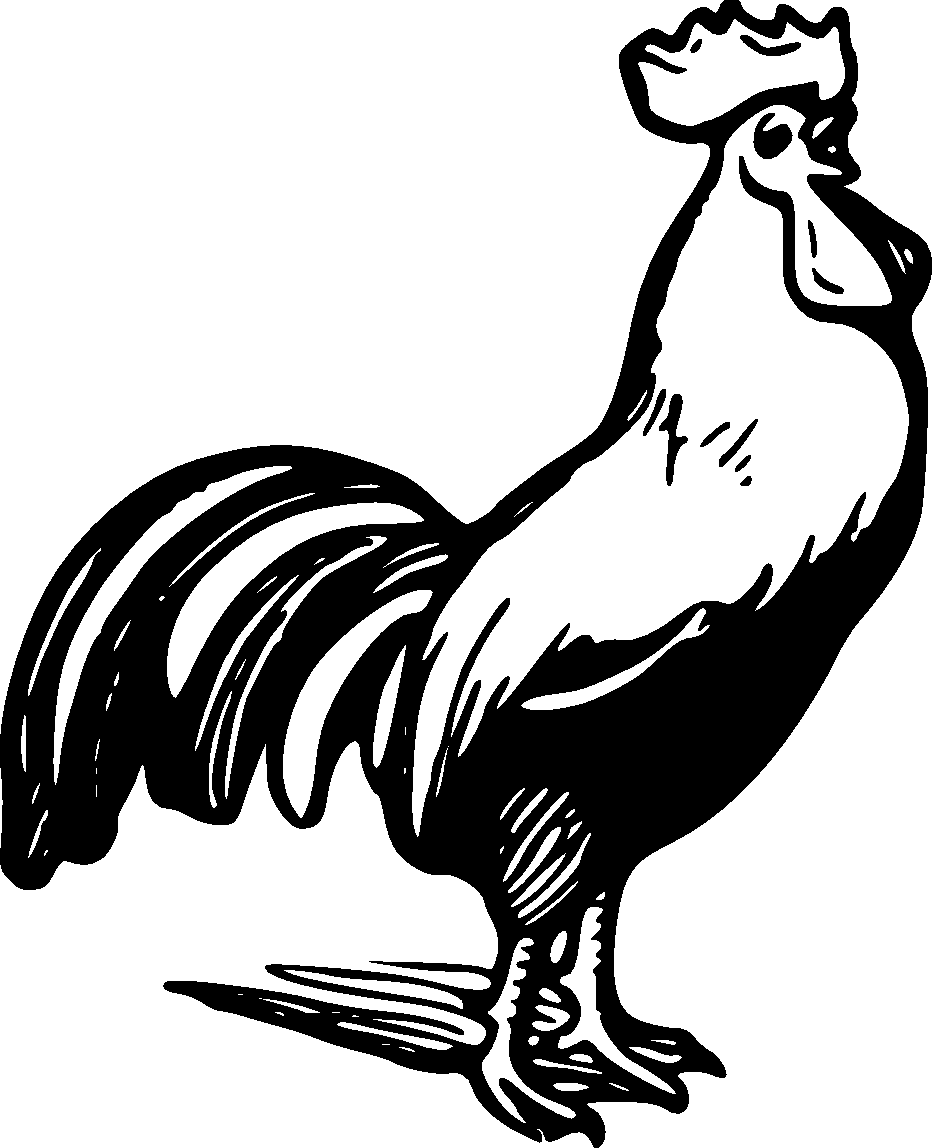
\includegraphics[height=0.9em]{coq.pdf}}
\newcommand{\CoqSymbol}{\raisebox{-.2ex}{\BareCoqSymbol\,}}
\newcommand{\Coqed}{\hfill\CoqSymbol}

\newcommand{\BareInvCoqSymbol}{
\includegraphics[height=0.9em]{inv_coq.png}}
\newcommand{\InvCoqSymbol}{\raisebox{-.2ex}{\BareInvCoqSymbol\,}}

%%%%
% Typerules
\newcommand{\textgraybox}[1]{\boxed{#1}}
\newdimen\zzfontsz
\newcommand{\fontsz}[2]{\zzfontsz=#1%
{\fontsize{\zzfontsz}{1.2\zzfontsz}\selectfont{#2}}}
\newcommand{\mathsz}[2]{\text{\fontsz{#1}{$#2$}}}
\newcommand{\instsymColon}{%
     \raisebox{-0.09ex}{\text{\normalfont{:}}}}
\newcommand{\judgboxfontsize}[1]{%
        \mathsz{11pt}{#1}%
}
\newcommand{\judgbox}[2]{%
      {\raggedright \textgraybox{\ensuremath{\judgboxfontsize{#1}}}\!%
        \fontsz{9pt}{\begin{tabular}[c]{l} #2 \end{tabular}} %
}}
\newcounter{typerule}
\crefname{typerule}{rule}{rules}

\newcommand{\typeruleInt}[5]{%
	\def\thetyperule{#1}%
	\refstepcounter{typerule}%
	\label{tr:#4}%
	%
  \ensuremath{\begin{array}{c}#5 \inference{#2}{#3}\end{array}}
}
\newcommand{\typerule}[4]{%
  \typeruleInt{#1}{#2}{#3}{#4}{\textsf{\scriptsize ({#1})} \\      }
}
\newcommand{\typerulenolabel}[3]{%
	\def\thetyperule{#1}%
	\refstepcounter{typerule}%
  \ensuremath{\begin{array}{c} \inference{#2}{#3}\end{array}}
}
\newcommand{\typerulederiv}[3]{%
  \ensuremath{\begin{array}{c} \inference{#2}{#3} #1\end{array}}
}

%%%%
% Language-specific definitions
% names of properties
\newcommand{\tmssafe}{\ensuremath\operatorname{tms}}
\newcommand{\smssafe}{\ensuremath\operatorname{sms}}
\newcommand{\mssafe}{\ensuremath\operatorname{ms}}
\newcommand{\scctsafe}{\ensuremath\operatorname{scct}}
\newcommand{\msscctsafe}{\ensuremath\operatorname{msscct}}

% Languages
\newcommand{\Ltms}{\ensuremath\src{L_{\tmssafe}}}
\newcommand{\Ltrg}{\ensuremath\trg{L}}
\newcommand{\Lms}{\ensuremath\irl{L_{\mssafe}}}
\newcommand{\Lscct}{\ensuremath\obj{L_{\scctsafe}}}

% Traces
\newcommand{\event}[1][]{a#1}
\newcommand{\absevent}[1][]{\ensuremath\bm{\event[#1]}}
\newcommand{\emptyevent}{\ensuremath\varepsilon}
\newcommand{\trace}[1][]{\ensuremath\overline{a#1}}
\newcommand{\class}[1][]{\ensuremath\mb{C}}
\newcommand{\lift}[1]{\ensuremath\lfloor\xspace{#1}\xspace\rfloor}
\newcommand{\hole}[1]{\ensuremath{\left[#1\right]}}
\newcommand{\ev}[1]{\text{#1}}
\newcommand{\absev}[1]{\ensuremath\bm{#1}}
\newcommand{\abstrace}[1][]{\ensuremath\bm{\trace[]}#1}
\newcommand{\absterm}{\ensuremath\lightning{\kern-5.5pt}\lightning}

% Trace Relations
\newcommand{\traceagree}[4][^*]{\ensuremath{#3}\cong_{#2}#1{#4}}
\newcommand{\tmstraceagree}[3][^*]{\traceagree[#1]{\tmssafe}{#2}{#3}}
\newcommand{\smstraceagree}[3][^*]{\traceagree[#1]{\smssafe}{#2}{#3}}
\newcommand{\mstraceagree}[3][^*]{\traceagree[#1]{\mssafe}{#2}{#3}}
\newcommand{\sccttraceagree}[3][^*]{\traceagree[#1]{\scctsafe}{#2}{#3}}

% Monitors
\newcommand{\monitor}[1][]{\ensuremath T#1}
\newcommand{\tmsmonitor}[1][]{\monitor[_{TMS}{#1}]}
\newcommand{\smsmonitor}[1][]{\monitor[_{SMS}{#1}]}
\newcommand{\scctmonitor}[1][]{\monitor[_{sCCT}{#1}]}
\newcommand{\msmonitor}[1][]{\monitor[_{MS}{#1}]}
\newcommand{\monitorcheck}[4][{\kern-3.5pt}^*]{%
  \vdash\xspace{#2}\xspace \xrsquigarrow{#4}{#1}\xspace{#3}\xspace%
}
\newcommand{\monsafe}[2]{\ensuremath\vdash_{mon}{#1}:{#2}}

\newcommand{\abssecuritytag}[1][]{\ensuremath\bm{\sigma}#1}

\newcommand{\montmssafe}[1]{\monsafe{#1}{\tmssafe}}
\newcommand{\monsmssafe}[1]{\monsafe{#1}{\smssafe}}
\newcommand{\monmssafe}[1]{\monsafe{#1}{\mssafe}}
\newcommand{\monscctsafe}[1]{\monsafe{#1}{\scctsafe}}
\newcommand{\monmsscctsafe}[1]{\monsafe{#1}{\msscctsafe}}

% Languages
\newcommand{\LTMS}{\src{L_{TMS}}}
\newcommand{\LT}{\trg{L}}
\newcommand{\LMS}{\irl{L_{MS}}}
\newcommand{\LCCT}{\obj{L_{sCCT}}}

\newcommand{\bnfdef}{\ensuremath{\mathrel{::=}}}

% Substitution
\newcommand{\subst}[2]{\ensuremath \hole{#1\text{ for }#2}}
\newcommand{\substvar}[1][]{\ensuremath \gamma#1}
\newcommand{\substlist}[1][]{\ensuremath \overline{\gamma#1}}

\newcommand{\partialeval}[2]{\ensuremath \operatorname{\mathtt{mix}}(#1, #2)}

% Predefined Sets
\newcommand{\nat}{\ensuremath\mb{N}}

% Types
\newcommand{\natt}{\ensuremath\mb{N}_t\xspace}
\newcommand{\ptrqual}[1][]{\ensuremath\xspace q#1\xspace}
\newcommand{\fullq}{1\xspace}
\newcommand{\halfq}{\sfrac{1}{2}\xspace}
\newcommand{\ptrn}[1][\ptrqual]{\ensuremath\xspace ref_{#1}\ \natt\xspace}
\newcommand{\wptr}{\ensuremath\ptrn[\halfq]\xspace}
\newcommand{\ptr}{\ensuremath\ptrn[\fullq]\xspace}
\newcommand{\type}[1][]{\ensuremath\tau#1\xspace}
\newcommand{\typenv}[1][]{\ensuremath\Gamma#1\xspace}

% Terms
\newcommand{\wrapkeyword}[2][]{\ensuremath{#1{#2}}}
\newcommand{\expr}[1][]{e#1\xspace}
\newcommand{\ectx}[1][]{K#1\xspace}
\newcommand{\finalexpr}[1][]{f#1\xspace}
\newcommand{\valueexpr}[1][]{v#1\xspace}
\newcommand{\lbinop}[3][]{\ensuremath {#2}{#1{\oplus}}{#3}\xspace}
\newcommand{\lget}[3][]{\ensuremath #2{#1{[}}{#3}{#1{]}}\xspace}
\newcommand{\lset}[4][]{\ensuremath #2{#1{[}}{#3}{#1{]\leftarrow}}#4\xspace}
\newcommand{\lnew}[3][]{\ensuremath \wrapkeyword[#1]{new}\ #2\ {#1{[}}#3{#1{]}}\xspace}
\newcommand{\llet}[4][]{\ensuremath \wrapkeyword[#1]{let}\ #2 {#1{=}} #3\ \wrapkeyword[#1]{in}\ #4\xspace}
\newcommand{\ldelete}[2][]{\ensuremath \wrapkeyword[#1]{delete}\ #2\xspace}
\newcommand{\lreturn}[2][]{\ensuremath \wrapkeyword[#1]{return}\ #2\xspace}
\newcommand{\lcall}[3][]{\ensuremath \wrapkeyword[#1]{call}\ #2\ #3\xspace}
\newcommand{\lifz}[4][]{\ensuremath \wrapkeyword[#1]{ifz}\ #2\ \wrapkeyword[#1]{then}\ #3\ \wrapkeyword[#1]{else}\ #4\xspace}
\newcommand{\labort}[1][]{\ensuremath \wrapkeyword[#1]{abort()}\xspace}
\newcommand{\lispoisoned}[2][]{\ensuremath #2\ \wrapkeyword[#1]{is\ }{#1{\poisoned}}\xspace}
\newcommand{\lpair}[3][]{\ensuremath {#1{\langle}} #2 {#1{;}} #3 {#1{\rangle}} \xspace}
\newcommand{\lproja}[2][]{\ensuremath {#2}{#1{.0}} \xspace}
\newcommand{\lprojb}[2][]{\ensuremath {#2}{#1{.1}} \xspace}
\newcommand{\lhast}[3][]{\ensuremath {#2}\ \wrapkeyword[#1]{has}\ #3 \xspace}
\newcommand{\lwrdoit}[2][]{\ensuremath \wrapkeyword[#1]{wrdoit}\ #2\xspace}
\newcommand{\lrddoit}[3][]{\ensuremath \wrapkeyword[#1]{rddoit}\ #2\ \wrapkeyword[#1]{in}\ #3\xspace}
\newcommand{\function}[1][]{F#1\xspace}
\newcommand{\lfunction}[4][]{\ensuremath\wrapkeyword[#1]{fn}\ {#2}\ {#3}\ {#1{:=}}\ #4\xspace}
\newcommand{\prog}[3][]{\ensuremath\wrapkeyword[#1]{\langle}\ #2; #3\wrapkeyword[#1]{\rangle}\xspace}

% Compiler
\newcommand{\rtp}[2]{\ensuremath\vdash{#1}:{#2}}
\newcommand{\ccbase}[1][]{\ensuremath\gamma{#1}}
\newcommand{\cc}[3][]{\ensuremath{\ccbase[#1]}^{#2}_{#3}\xspace}
\newcommand{\cca}{\ensuremath\cc{\Ltms}{\Ltrg}}
\newcommand{\ccb}{\ensuremath\cc{\Ltrg}{\Lms}}
\newcommand{\ccdce}{\ensuremath\cc[_{\gls{dce}}]{\Lms}{\Lms}}
\newcommand{\cccf}{\ensuremath\cc[_{\gls{cf}}]{\Lms}{\Lms}}
\newcommand{\ccscct}{\ensuremath\cc{\Lms}{\Lscct}}
\newcommand{\ccmsscct}{\ensuremath\cc{\Ltms}{\Lscct}}

% Backtranslation
\newcommand{\backbase}[1][]{\ensuremath\wp#1}
\newcommand{\backt}[3][]{\ensuremath{}^{#2}_{#3}\backbase[#1]}

% Satisfaction
\newcommand{\contextvar}[1][]{C#1}
\newcommand{\progvar}[1][]{p#1}
\newcommand{\wholeprogvar}[1][]{w#1}
\renewcommand{\class}[1][]{\mathbb{C}#1}
\newcommand{\link}[2]{\ensuremath\operatorname{link}\left({#1};{#2}\right)}
\newcommand{\behav}[1]{\ensuremath\operatorname{behav}\left({#1}\right)}
\newcommand{\sat}[2]{\ensuremath\vdash{#1}:{#2}}
\newcommand{\rsat}[2]{\ensuremath\vdash_R{#1}:{#2}}

% State
\newcommand{\securitytag}[1][]{\ensuremath\sigma#1}
\newcommand{\sandboxtag}[1][]{t#1}
\newcommand{\ctx}{\text{ctx}}
\newcommand{\comp}{\text{comp}}
\newcommand{\loc}[1][]{\ensuremath l#1}
\newcommand{\poison}{\ensuremath\rho}
\newcommand{\poisoned}{\ensuremath\text{\Biohazard}}
\newcommand{\poisonless}{\ensuremath\square}
\newcommand{\store}[1][]{\ensuremath\Delta#1}
\newcommand{\storeel}[5]{\ensuremath #1\mapsto\tup{#2}{#3,#4,#5}}
\newcommand{\comm}[1][]{\ensuremath c#1}
\newcommand{\ctxtocomp}{\ensuremath\xspace ? \xspace}
\newcommand{\comptoctx}{\ensuremath\xspace ! \xspace}
\newcommand{\nocomm}{\ensuremath\xspace \varnothing \xspace}
\newcommand{\heap}[1][]{\ensuremath H#1}
\newcommand{\ectxstack}[1][]{\ensuremath\overline{\ectx#1}}
\newcommand{\library}[1][]{\ensuremath\Xi#1}
\newcommand{\commlib}[1][]{\ensuremath\xi#1}
\newcommand{\cfstate}[1][]{\ensuremath\Psi#1}
\newcommand{\memstate}[1][]{\ensuremath\Phi#1}
\newcommand{\statevar}[1][]{\ensuremath\Omega#1}
\newcommand{\rtt}[2]{\ensuremath #1 \triangleright #2}
\newcommand{\growh}[2]{\ensuremath #1 \ll #2}
\newcommand{\seth}[3]{\ensuremath #1(#2 \mapsto #3)}

% Various Judgements
\newcommand{\fresh}[2]{\ensuremath{#1}\vdash{#2}\xspace\operatorname{fresh}\xspace}
\newcommand{\tcheck}[3]{\ensuremath{#1}\vdash{#2}:{#3}\xspace}
\newcommand{\notowned}[1]{\ensuremath\vdash{#1}\xspace\operatorname{not-owned}\xspace}
\newcommand{\typenvsplit}[2]{\ensuremath {#1}\odot{#2}\xspace}
\newcommand{\hastype}[2]{\ensuremath{#1}:{#2}\xspace}
\newcommand{\inttype}[1]{\ensuremath\vdash{#1}\operatorname{int-\type}\xspace}

\newcommand{\thelocmap}{\ensuremath\delta\xspace}
\newcommand{\locmapsto}[2]{\ensuremath\thelocmap({#1})={#2}\xspace}

% Filters
\newcommand{\filter}[4][]{\ensuremath \operatorname{Proj}^{#1}_{#2}\left({#3}, {#4}\right)\xspace}
\newcommand{\msfilterLtms}[2][{\thelocmap}]{\ensuremath\filter[{\Ltms}]{}{#1}{#2}}
\newcommand{\msfilterLms}[2][{\thelocmap}]{\ensuremath\filter[{\Lms}]{}{#1}{#2}}
\newcommand{\msfilterL}[2][{\thelocmap}]{\ensuremath\filter[{\Ltrg}]{}{#1}{#2}}
\newcommand{\scctfilterLms}[2][{\thelocmap}]{\ensuremath\filter[{\Lms}]{}{#1}{#2}}
\newcommand{\scctfilterLscct}[2][{\thelocmap}]{\ensuremath\filter[{\Lscct}]{}{#1}{#2}}

% Steps
\newcommand{\isval}[1]{\ensuremath\vdash{#1}\xspace\operatorname{is-val}\xspace}
\newcommand{\runtimetermvar}[1][]{r#1}
\newcommand{\stepto}[4][{\kern-4.5pt}^*]{\ensuremath{#2}\xrightarrow{#4}{}\xspace{#1}\xspace{#3}\xspace}
\newcommand{\stepton}[4][n]{\ensuremath{#2}\xrightarrow{#4}{}{\kern-3.5pt}^{#1}\xspace{#3}\xspace}

\newcommand{\pstepto}[3]{\ensuremath{#1}\xrightarrow{#3}_p{}\xspace{#2}\xspace}
\newcommand{\estepto}[4][{\kern-4.5pt}^*]{\ensuremath{#2}\xrightarrow{#4}#1_{\operatorname{ectx}}\xspace{#3}\xspace}
\newcommand{\estepton}[4][n]{\ensuremath{#2}\xrightarrow{#4}_{\operatorname{ectx}}{}{\kern-14.5pt}^{#1\ \ \ \;}\xspace{#3}\xspace}
\newcommand{\progstepto}[3]{\ensuremath{#1}\xRightarrow{#3}{#2}}


% allow page breaks inside multiline alignment displays
\allowdisplaybreaks

\Crefname{exampleenv}{Example}{Examples}

\theoremstyle{definition}
\newtheorem{exampleenv}{Example}[section]
\newtheorem{lemma}{Lemma}[section]
\newtheorem{theorem}{Theorem}[section]
\newtheorem{corollary}{Corollary}[section]
\newtheorem{definition}{Definition}[section]

\loadglsentries{acronyms}
\makeglossaries

\AtBeginDocument{%
  \providecommand\BibTeX{{%
    \normalfont B\kern-0.5em{\scshape i\kern-0.25em b}\kern-0.8em\TeX}}}
\makeatletter
\newcommand{\linebreakand}{%
  \end{@IEEEauthorhalign}
  \hfill\mbox{}\par
  \mbox{}\hfill\begin{@IEEEauthorhalign}
}
\makeatother

\renewcommand\thelinenumber{\color{red}\arabic{linenumber}}
\begin{document}
\linenumbers

\title{Secure Composition \\ of Robust and Optimising Compilers}

\author{}
% Matthis Kruse\orcidID{0000-0003-4062-9666}
% \and
% Michael Backes
% \and
% Marco Patrignani
% }
% \authorrunning{M. Kruse et al.}

\maketitle

\begin{abstract}
% \MPpost{
%   this abstract fails in setting up the robustness argument.
%   it'll be a good exercise for you to take inspiration from this, but then write something as concise but with a more direct focus on robust properties
% }
% context
To ensure that secure applications do not leak their secrets, they are required to uphold several security properties such as spatial and temporal memory safety as well as cryptographic constant time.
% need
Existing work shows how to enforce these properties individually, in an architecture-independent way, by using secure compiler passes that each focus on an individual property.
% task
Unfortunately, given two secure compiler passes that each preserve a possibly different security property, it is unclear what kind of security property is preserved by the composition of those secure compiler passes.
%there is no way to tell what kind of security property will the composition of those secure compilers preserve.

% object
This paper is the first to study what security properties are preserved across the composition of different secure compiler passes.
% findings
Starting from a general theory of property composition for security-relevant properties (such as the aforementioned ones), this paper formalises a theory of composition of secure compilers.
Then, it showcases this theory on a secure multi-pass compiler that preserves the aforementioned security-relevant properties.
% conclusion
Crucially, this paper derives the security of the multi-pass compiler from the composition of the security properties preserved by its individual passes, which include security-preserving as well as optimisation passes.
% 
From an engineering perspective, this is the desirable approach to building secure compilers.


  % \MKin{context}
  % Memory safety necessitates secrecy, since breaking it can lead to an arbitrarily large attack space, i.e., from simply reading a secret up to alteration of control-flow in order to execute arbitrary code.
  % However, secrecy cannot be achieved with just memory safety alone, since, e.g., private data could be leaked by differences in execution time for varying program inputs.
  % This leakage is avoidable by ensuring that programs are cryptographic constant time, i.e., different inputs do not change execution time.
  % Prior work has shown that strategies to ensure cryptographic constant time can be rendered useless, since a compiler may simply optimize them away.
  % \MKin{need}
  % This is why secure compilation is an integral ingredient to achieve security, because a secure compiler guarantees (formally) that properties that hold in the source, also hold in the target. %% mention attacker? the text describes correctness
  % \MKin{task}
  % Unfortunately, it is an open question whether secure compilers can be engineered in a modular way.
  % Ideally, compiler engineers develop two different compilation passes, one that ensures memory safety and another one that is security preserving with respect to cryptographic constant time. %, because this style of engineering is well-established for its simplifying divide-and-conquer approach as well as enhanced reusability.
  % \MKin{object+findings}
  % This paper answers that question positively: The composition of compilers that are secure with respect to some security-properties yields the intersection of these properties.
  % \MKin{object}
  % This article discusses different variants of compositions of secure compilers and instantiates parts of these results in a case-study.
  % To this end, it presents an optimizing, secure compilation chain that preserves both memory safety and cryptographic constant time.
  % \MKin{conclusion}
  % The compositionality results enable modular proofs for the presented, secure compiler. % that is secure with respect to both memory safety and cryptographic constant time.
  % Some results of this work are implemented in the Coq proof assistant.

\begin{center}\small\it
	{This paper uses syntax highlighting accessible to both colourblind and black \& white readers.
	% ~\cite{patrignani2020use}.
% 	% Specifically, it makes use of a $\src{blue}$, $\src{sans\text{-}serif}$ font for a $\src{source}$,
% 	% a $\trg{red}$, $\trg{bold}$ font for an $\trg{intermediate}$,
% 	% and a $\obj{green}$, $\obj{teletype}$ font for a $\obj{target}$ language.
	}
\end{center}
\end{abstract}

\begin{IEEEkeywords}
  memory-safety, cryptographic constant-time, secure compilation, robustness
\end{IEEEkeywords}

\section{Introduction\pages{4}}\label{sec:introduction}

% \gls*{ms} is a security property that ensures that there are no out-of-bounds accesses as well as no reads or writes to uninitialised memory.
% Programs that do not attain memory safety, can easily have their private data be leaked to attackers or be corrupted~\cite{lemay2021ccc}.
% Because of this, \gls*{ms} is a requirement for programs to attain an even stronger security property, namely \gls*{cct}.
% Programs that attain \gls*{cct} are secure with respect to timing attacks, and this is the gold standard for secure applications, including cryptographic ones, since timing attacks can expose secrets via a simple performance analysis~\cite{kocher1996timing}.
% Timing attacks have become more and more relevant recently, especially given the era of cloud-computing~\cite{aviram2010cloudtime,kumar2019cloudsecsurvey}, where programs share the same hardware but are supposed to run in a sandboxed environment that does not leak secrets.
% Unfortunately, several attacks within such a cloud environment have been demonstrated as viable strategies to extract secrets~\cite{mehmet2015getoff,flowers2022zeroday,atya2019catchme,venkatanathan2015placevul}.

% Even though mitigations for such attacks exist~\cite{bond2017vale,almeida2017jasmin}, some compilers may optimise these mitigations away~\cite{barthe2018sec}.
% This is of course not what programmers expect and to ensure such mitigations persist in the compiled code, one can use a {\em secure} compilers.
% More generally, secure compilers should preserve security properties even when the program runs in a hostile context such as the cloud one, i.e., where it interacts with other possibly malicious programs.
% An example of such secure compilers are those that ascribe to the theory of robust compilation~\cite{abate2019jour,abate2021extacc,patrignani2021rsc}, which takes this interaction between components and potentially malicious contexts into account.

% Unfortunately, it is unclear if and how robust compilation supports compositionality, and compilation passes are typically developed as a standalone module to be plugged into a compilation pipeline and composed with other passes.
% Different kinds of compilation passes exist, e.g., there are usually several compilation passes that perform optimisations~\cite{lattner2004llvm,googlev8,androidstudio,kuepper2023cryptopt,manjikian1997fusion,wegman1991ccp} or source-code instrumentations~\cite{nagarakatte2009soft,nagarakatte2010cets,akritidis2009baggy,dhumbumroong2020boundwarden,jung2021pico,nam2019framer,shankaranarayana2023tailcheck,younan2010paricheck,zhou2023fatptrs,bond2017vale,almeida2017jasmin,kuepper2023cryptopt,cauligi2019fact} that enforce that the compiled program fulfils a property of interest.
% Without a framework for composing secure compiler passes, it is not possible to enable separation of concerns, e.g., to have a secure compilation pass that ensures \gls*{ms} that is developed independently of another secure pass for \gls*{cct} as suggested before and as showcased in \Cref{ex:strncpy}.
% \MPpost{
%   this intro does a poor job at introducing the robust compilation argument.
%   perhaps it'd be best to start from robust properties, which motivates the use of robust compilers?
%   idk
%   as for the abstract, this is a good starting point for you to make a better intro
% }

\gls*{ms} is a security property obtained by composing \gls*{sms}, which ensures array accesses are all within bounds, and \gls*{tms}, which ensures pointers are only used when they are valid~\cite{azevedo2018meaningsofms,jim2002cyclone,necula2005ccured,nagarakatte2010cets,nagarakatte2009soft,akritidis2009baggy,michael2023mswasm}.
\gls*{cct} is a security property that ensures sensitive data is not leaked via timing side-channels~\cite{kocher1996timing}.
Together, \gls*{sms}, \gls*{tms}, \gls*{scct}, an enforceable overapproximation of \gls*{cct}, and \gls*{ss}, yield \gls*{mssscct}, which is the gold standard of security properties for secure applications.
Programs attaining \gls*{mssscct} do not leak sensitive data either through erroneous memory accesses, nor through timing side-channels, even under speculative execution.
As discussed in \Cref{ex:strncpy}, these security properties can be enforced by compiler passes~\cite{bond2017vale,almeida2017jasmin}, to ensure programmers need not be aware of the architectural details of where their code will run.

\begin{exampleenv}[strncpy]\label{ex:strncpy}
Consider the \texttt{C} function \texttt{strncpy} that copies a null-terminated string \texttt{src} into \texttt{dst} up to a length of \texttt{n}.
% Assume that the length of the array pointed by \texttt{dst} is at least \texttt{n}, and \texttt{src} is terminated by \texttt{'\textbackslash 0'}.
% Even under these assumptions, there is a 
This function is subject to a subtle \gls*{sms} vulnerability: the bounds check \texttt{i < n} should happen {\it before} the access to memory location \texttt{src[i]}: otherwise
% If \texttt{n} is at least as large as the length of the array \texttt{src}, 
the memory location past the last element will be leaked to an attacker.
\begin{lstlisting}[language=c,basicstyle=\footnotesize\ttfamily,morekeywords={size_t}]
void strncpy(size_t n, char *dst, char *src) {
  for(size_t i = 0; src[i] != '\0' && i < n; ++i) {
    dst[i] = src[i];
  }
}
\end{lstlisting}

To prevent this vulnerability, one can use a compilation pass that enforces \gls*{sms}, such as Softbounds~\cite{nagarakatte2009soft} or BaggyBounds~\cite{akritidis2009baggy}.
The most naive solution in this case is to insert bounds-checks in front of every access to memory.

Because of timing attacks, addressing \gls*{sms} is not enough to make \texttt{strncpy} secure.
In fact, the loop can terminate early, as soon as the string-terminating character \texttt{'\textbackslash 0'} is encountered, thus making program execution time proportional to the length of the array pointed by \texttt{src}, and violating the \gls*{cct} property.
% Often, programmers rewrite programs like these to have loops that run with a fixed number of iterations.
Also in this case there exist compiler passes that can rewrite such programs into \gls*{cct} ones~\cite{cauligi2019fact}.
 % so that they are no longer vulnerable to timing attacks.
%
Alas, code is not run in isolation, so a malicious attacker could supply code that interacts with \texttt{strncpy} and trigger a violation of either \gls*{ms} or \gls*{cct} by calling \texttt{strncpy} with an argument for \texttt{src} that points to uninitialised memory.
This would, in turn, triggering a series of reads from uninitialised memory, which is an immediate \gls*{ms} violation with devastating real-world consequences~\cite{uninit-0,uninit-1,uninit-2,uninit-3,uninit-4}.
% An easy fix to sidestep this is to use non-nullable pointers as parameters instead, e.g., as presented in Cyclone~\cite{jim2002cyclone}.

Robust compilers~\cite{abate2019jour} are a form of secure compilers that preserve security properties even in the presence of arbitrary attackers interacting with compiled code.
Thus, robust compilers can be used to prevent vulnerabilities resulting from uninitialised memory (as well as many other ones), e.g., by targeting capability-based languages such as CHERI~\cite{woodruff2014CHERI}, Arm Morello~\cite{arm-morello}, or MSWasm~\cite{michael2023mswasm}, where the compiler relies on capabilities to check that pointers are always initialised.
\end{exampleenv}

% To ensure these compiler-preserved properties still hold even in the presence of arbitrary attackers interacting with compiled code, one can use secure compilers in the form of robust compilers~\cite{abate2019jour,abate2021extacc,patrignani2021rsc}.

Unfortunately, given secure compiler passes that each preserve a possibly different security property, there is no way to tell what kind of security property will the composition of those secure compilers preserve.
% Different kinds of compilation passes exist, e.g., there are usually several compilation passes that perform optimisations~\cite{lattner2004llvm,googlev8,androidstudio,kuepper2023cryptopt,manjikian1997fusion,wegman1991ccp} or source-code instrumentations~\cite{nagarakatte2009soft,nagarakatte2010cets,akritidis2009baggy,dhumbumroong2020boundwarden,jung2021pico,nam2019framer,shankaranarayana2023tailcheck,younan2010paricheck,zhou2023fatptrs,bond2017vale,almeida2017jasmin,kuepper2023cryptopt,cauligi2019fact} that enforce that the compiled program fulfils a property of interest.
Worse, without a framework for composing secure compiler passes, it is not possible to enable separation of concerns, e.g., to have a secure compilation pass that ensures \gls*{ms} that is developed independently of another secure pass for \gls*{cct}, that is developed independently of other passes, such as optimisations.


This paper introduces a framework for reasoning about the composition of secure and optimising compiler passes akin to those of \Cref{ex:strncpy} and it showcases the power of this framework by instantiating it on a multi-pass compilation chain.
To this end, this paper first discusses how to compose security properties, such as \gls*{tms} and \gls*{sms} into \gls*{ms}, and then adding \gls*{scct} to the mix to obtain \gls*{msscct}.
Then, this paper defines compiler composition and formalises that given two passes that securely preserve two (possibly distinct) properties, their composition securely preserves the composition of those properties.
The paper then defines several secure compiler passes, where each is either preserving a different security property (\gls*{tms}, \gls*{sms}, \gls*{scct}, \gls*{ss}) or performing a security-preserving optimisation, (e.g., applying \gls*{cf} or \gls*{dce}).
Finally, this paper shows that composing these secure compiler passes into a multi-pass compilation chain results in the end-to-end preservation of \gls*{mssscct}.
Crucially, this paper derives the security of the multi-pass compiler from the composition of the security properties preserved by its individual passes.
% Crucially, this end-to-end security preservation is obtained by composing the security property preserved by each individual pass, as dictated by the framework of this paper.
This result showcases how the framework allows the kind of formal security reasoning that compiler writers already want (and already do), obtaining precise, compositional security reasoning while providing minimal (and modular) proof effort.
%
In summary, this paper makes the following contributions:
\begin{itemize}
  \item %
        %\Cref{sec:compcomp} studies different forms of secure compiler compositions.
        This paper takes the secure compilation framework of Abate et al.~\cite{abate2021extacc} and extends it for compositionality. (\Cref{sec:sequential}).
        %Concretely, it investigates upper and lower compositions, as well as the sequential composition.
        %For this, this paper studies compiler composition as well as compilers with multiple input languages or multiple output ones, as used in existing compilation chains.
        %
        This paper proves that starting from two compilers that preserve two (possibly distinct) properties, their composition preserves roughly the intersection of those properties.
        % For example, a compiler that is secure with respect to \gls*{tms} can be composed with a compiler that is secure with respect to \gls*{sms}, resulting in a compiler that is secure with respect to \gls*{ms}.
        % 
        From this, the paper proves that the order of composition of sequential compiler passes is irrelevant for security.
        % 
        This is crucial for reordering individual optimisation passes and thus generating secure and efficient code.
        %
        %Finally, this paper extends parts of the compositionality framework to support different trace-models between compilation passes.

  \item %
        This paper presents a case-study with five programming languages showcasing the previous contribution (\Cref{sec:casestud:defs,sec:casestud:rtp}).
        To this end, it presents a compilation chain consisting of six passes, two of which are well-known optimisations \gls*{dce} and \gls*{cf}, that ultimately preserve \gls*{mssscct} by means of composing the individual, secure passes concerning \gls*{tms}, \gls*{sms}, \gls*{scct}, and \gls*{ss}, respectively.
        %Furthermore, the chain includes two optimisation passes: One performs \gls*{dce} and the other \gls*{cf}.
        The formalisation of this case study showcases the power of the presented framework: The divide-and-conquer approach to software engineering is a viable strategy even for the development of secure compilers.
%        This demonstrates that the usage of the presented framework is both simpler and more expressive compared to one monolithic security proof of the whole compilation chain.

  \item %
        The considered compilation passes are analyzed in terms of their compatibility with each other (\Cref{sec:formalities}).
        In doing so, the paper provides formal insights into some technicalities of the concrete proofs necessary as technical setup to reap the benefits of the presented compositionality framework.

  \item The key contributions of this paper are formalised in the Coq proof assistant and the paper indicates this with \CoqSymbol.
\end{itemize}
% 
This paper starts by introducing relevant notions of security properties and secure compilation (\Cref{sec:background}),
and discusses related work (\Cref{sec:relwork}) before concluding (\Cref{sec:concl}).

\contribution{Open Source \& Technical Report} A technical report with the omitted formal details, lemmas and proofs, as well as the Coq formalisation are available as supplementary material.
% \MKin{cite/link}

\section{Background: Security Properties and Secure Compilers\pages{1}}\label{sec:background}

To introduce the security argument of this paper, this section first presents the concepts of (security) properties, of their satisfaction, and of their robust satisfaction (i.e., satisfaction in the presence of an active attacker; \Cref{subsec:bg:tprop}).
Then, borrowing from existing work~\cite{abate2019jour,abate2021extacc}, the section introduces secure compilers as compilers that preserve robust property satisfaction (\Cref{subsec:bg:rtp}).

\subsection{Properties and (Robust) Satisfaction}\label{subsec:bg:tprop}

This paper employs the security model where programs are written in a language whose semantics emits events $\event$.
Events include security-relevant actions (e.g., reading from and writing to memory, as detailed in \Cref{sec:compprop}) and the unobservable event $\emptyevent$.
As programs execute, their emitted events are concatenated in traces $\trace$, which serve as the description of the behaviour of a program.%
\footnote{
Throughout the paper, sequences are indicated with an overbar (i.e., $\trace$), empty sequences with $\hole{\cdot}$, and concatenation of sequences $\trace[_{1}],\trace[_{2}]$ as $\trace[_{1}]\cdot\trace[_{2}]$.
Prepending elements to sequences uses the same notation: $\event\cdot\trace$.
}

Properties $\pi$ are sets of traces of admissible program behaviours, ascribing what said property considers valid.
The set of all properties can be partitioned into different {\em classes} ($\class$), i.e., safety, liveness, and neither safety nor liveness~\cite{clarkson2008hyper}.
A class is simply a set of properties and for the class of safety properties, it is decidable whether a trace satisfies a safety property with just a finite trace prefix.
The compositionality framework (\Cref{sec:compcomp}) presented in this paper considers arbitrary classes, while the case-study (\Cref{sec:casestud:rtp}) fixes them to concrete instances.
As an example, consider a trace describing an interaction with a memory where the deallocation of an address $\loc$ precedes a read at that address in memory: $\ev{Dealloc\ \loc}\cdot\ev{Read\ \loc\ 1729}\cdot\dots$.
This program behaviour is insecure with respect to a canonical notion of (temporal) memory safety dictating no use-after-frees of pointers~\cite{nagarakatte2010cets,azevedo2018meaningsofms}, because it reads from a memory location that was freed already.
The previous finite trace prefix is enough to decide that the trace does not satisfy \gls*{tms} and there is no way to append events to this prefix which would result in the trace being admissible.
In the following, the execution of a whole program $\wholeprogvar$ that terminates in state $\runtimetermvar$ according to the language semantics and produces trace $\trace$ is written as $\progstepto{\wholeprogvar}{\runtimetermvar}{\trace}$.
With this, property satisfaction is defined as follows:
\bul{whole programs $\wholeprogvar$ satisfy a property $\pi$} iff \iul{$\wholeprogvar$ yields a trace $\trace$} such that \oul{$\trace$ satisifies $\pi$} (\Cref{def:propsat}).

\begin{definition}[Property Satisfaction]\label{def:propsat}
    \bul{$\sat{\progvar}{\pi}$}
    $\isdef$
    if \iul{$\forall\runtimetermvar\ \trace,\progstepto{\progvar}{\runtimetermvar}{\trace}$},
    then \oul{$\trace\in\pi$}.
\end{definition}

Property satisfaction is defined on whole programs, i.e., programs without missing definitions.
Thus, from a security perspective, this considers only a passive attacker model, where the attacker observes the execution and, e.g., retrieves secrets from that.
To consider a stronger model similarly to what existing work does~\cite{abate2019jour,abate2021extacc,maffeis2008code-carrying,gordon2003authenticity,fournet2007authorization,bengtson2011refine,backes2014uniontyps,michael2023mswasm,swasey2017robust,sammler2019benefits}, the concept of satisfaction can be extended with {\em robustness}.
Robust satisfaction considers partial programs $\progvar$, i.e., components with missing imports, which cannot run until said imports are fulfilled.
To remedy this, {\em linking} takes two partial programs $\progvar[_{1}],\progvar[_{2}]$ and produces a whole program $\wholeprogvar$, i.e., $\link{\progvar[_{1}]}{\progvar[_{2}]}=\wholeprogvar$.
As typically done in works that consider the execution of partial programs~\cite{abate2019jour,devriese2018parametricity,patrignani2021rsc,korashy2021capableptrs,strydonck2019lincap,devriese2017modular,bowman2015noninterference,ahmed2011equivcps,patterson2017linkingtyps},
this paper assumes that whole programs are the result of linking partial programs referred to as {\em context} ($\ctx$) and {\em component} ($\comp$).
The context is an arbitrary program and thus has the role of an {\em attacker} that can interact with the component by means of whatever features the programming language has, and the component is what is security-relevant.
%In this work, the semantics of the programming language is expected to differentiate between the component and the context.
With this, \Thmref{def:propsat} can be extended as follows: for \bul{components $\progvar$ to robustly satisfy a property $\pi$}, take an \iul{attacker context $\contextvar$ and link it with $\progvar$}, \oul{the resulting whole program must satisfy $\pi$}.

\begin{definition}[Robust Satisfaction]\label{def:proprsat}
  % \begin{nscenter}
  \bul{$\rsat{\progvar}{\pi}$}
  $\isdef$ \iul{$\forall \contextvar\ \wholeprogvar$, if $\link{\contextvar}{\progvar}=\wholeprogvar$}, then \oul{$\sat{\wholeprogvar}{\pi}$}.
  % \end{nscenter}
\end{definition}

% \begin{exampleenv}[Double Free in Bluetooth Subsystem]
%   Consider \texttt{CVE-2021-3564}~\cite{doublefree-bluetooth}, one of many submissions for a double-free vulnerability.
%   The vulnerability arises due to a race condition where the context-level function \texttt{hci\_cmd\_work} was not expected to behave maliciously, since it resides in the same source-code repository where the vulnerability occurs.
%   Nevertheless, the component-level code of \texttt{hci\_dev\_do\_open} is linked with \texttt{hci\_cmd\_work} and does not atomically check whether a pointer has been freed already:
%   Therefore, \texttt{hci\_dev\_do\_open} does not satisfy the no-double-frees property robustly, since there is an implementation for \texttt{hci\_cmd\_work} that leads to a violation of that property when linked with \texttt{hci\_dev\_do\_open}.
% \end{exampleenv}

\subsection{Secure Compilers}\label{subsec:bg:rtp}

A {\em compiler} ($\cc{\src{L}}{\trg{L}}$) translates syntactic descriptions of programs from a {\em source} ($\src{L}$) into a {\em target} ($\trg{L}$) programming language.
This translation is considered {\em correct} if it is semantics-preserving.
That is, for a whole program $\src{\wholeprogvar}$, the compiler should relate the $\src{L}$ semantics of $\src{\wholeprogvar}$ with the semantics of $\trg{L}$ of the compiled counterpart of $\src{p}$ in such a way that they are ''compatible''.
Unfortunately, correct compilers may be insecure compilers~\cite{patrignani2019survey,kennedy2006secure.net,abadi1999protect,ahmed2018dagstuhl} and programs translated by insecure compilers can violate security properties that the programmer assumes to hold.
This is why {\em robust preservation} is a good candidate as a compiler-level security property~\cite{abate2019jour}.

This paper uses a more general notion of robust preservation~\cite{abate2021extacc} that applies to compilers that use languages with different trace models. 
To this end, considering a source trace $\src{\trace}$ and a target trace $\trg{\trace}$, there is a relation ($\sim$) describing the effect of a corresponding compiler. 
\MKin{reference example from case study}
Using this relation, there are two projection functions: (1) the existential image $\tau_\sim\left(\src{\pi}\right)$ and (2) the universal image $\sigma_\sim\left(\trg{\pi}\right)$.
These projections map source-level (resp. target-level) properties to target-level (resp. source-level) properties. 
The case study of this paper exclusively uses the universal image, since some considered properties, such as \gls*{ss}, are not definable in a higher-level language that, e.g., does not model speculation.

Using these projection functions, the more general version of robust preservation is defined as follows~\cite{abate2021extacc}:
For a \bul{compiler $\cc{\src{L}}{\trg{L}}$ to robustly preserve a class of source properties $\src{\class}$}, if for any \rul{property $\src{\pi}$ of that class $\src{\class}$ and programs $\src{p}$ written in $\src{L}$} where \iul{$\src{\progvar}$ robustly satisfies $\src{\pi}$}, then \oul{the compilation of $\src{\progvar}$, $\cc{\src{L}}{\trg{L}}\left(\src{p}\right)$, must robustly satisfy $\tau_\sim\left(\src{\pi}\right)$}.

\begin{definition}[Robust Preservation with $\tau_\sim$]\label{def:rtp:tau}
  % $\;$\\
  % \vspace{-1em}
  % \begin{nscenter}
  % Compiler $\cc{\src{L}}{\trg{L}}$ robustly preserves $\class$, 
  \bul{$\rtptau{\cc{\src{L}}{\trg{L}}}{\src{\class}}{\sim}$}
  %, iff 
  $\isdef$
  \rul{$\forall \src{\pi}\in\src{\class}, \src{p}\in\src{L},$} if \iul{$\rsat{\src{\progvar}}{\src{\pi}}$}, then \oul{$\rsat{\cc{\src{L}}{\trg{L}}\left(\src{p}\right)}{\tau_\sim{\left(\src{\pi}\right)}}$}.
  % \end{nscenter}
\end{definition}
% 
Note that a class of properties $\class$ can represent just one property $\pi$ by lifting~\cite{clarkson2008hyper} that property to sets of properties, i.e., use the powerset of $\pi$ instead of $\pi$ itself.
Because of this, this paper may write $\rtptau{\cc{\src{L}}{\trg{L}}}{\src{\pi}}{\sim}$, even though $\src{\pi}$ is a property and not a class.
A similar construction can be applied to the projection functions.

Dually to \Cref{def:rtp:tau}, for a \bul{compiler $\cc{\src{L}}{\trg{L}}$ to robustly preserve a class of target properties $\trg{\class}$}, if for any \rul{property $\trg{\pi}$ of that class $\trg{\class}$ and programs $\src{p}$ written in $\src{L}$} where \iul{$\src{\progvar}$ robustly satisfies $\sigma_\sim\left(\trg{\pi}\right)$}, then \oul{the compilation of $\src{\progvar}$, $\cc{\src{L}}{\trg{L}}\left(\src{p}\right)$, must robustly satisfy $\trg{\pi}$}.

\begin{definition}[Robust Preservation with $\sigma_\sim$]\label{def:rtp:sigma}
  % $\;$\\
  % \vspace{-1em}
  % \begin{nscenter}
  % Compiler $\cc{\src{L}}{\trg{L}}$ robustly preserves $\class$, 
  \bul{$\rtpsig{\cc{\src{L}}{\trg{L}}}{\trg{\class}}{\sim}$}
  %, iff 
  $\isdef$
  \rul{$\forall \trg{\pi}\in\trg{\class}, \src{p}\in\src{L},$} if \iul{$\rsat{\src{\progvar}}{\sigma_\sim\left(\trg{\pi}\right)}$}, then \oul{$\rsat{\cc{\src{L}}{\trg{L}}\left(\src{p}\right)}{\trg{\pi}}$}.
  % \end{nscenter}
\end{definition}

A degenerate case where $\sim$ coincides with equality, i.e., the trace model is the same for both source and target programs, is the classic definition of robust preservation~\cite{abate2019jour}:

\begin{definition}[Robust Preservation]\label{def:rtp}
  % $\;$\\
  % \vspace{-1em}
  % \begin{nscenter}
  % Compiler $\cc{\src{L}}{\trg{L}}$ robustly preserves $\class$, 
  \bul{$\rtp{\cc{\src{L}}{\trg{L}}}{\class}$}
  %, iff 
  $\isdef$
  \rul{$\forall \pi\in\class, \src{p}\in\src{L},$} if \iul{$\rsat{\src{\progvar}}{\pi}$}, then \oul{$\rsat{\cc{\src{L}}{\trg{L}}\left(\src{p}\right)}{\pi}$}.
  % \end{nscenter}
\end{definition}

\section{Secure Composition}\label{sec:sequential}

Notably, real-world compilation chains also perform a series of (sequential) passes whose main purpose is not necessarily to translate from one language to another, but to, e.g., optimise the code or enforce a certain property.
Both examples can be seen in practice, e.g. as in the work of~\cite{nagarakatte2009soft,nagarakatte2010cets,akritidis2009baggy,wegman1991ccp,manjikian1997fusion} and many more.
% \MPin{survey to cite? this is a bit informal MK: hard to find a survey on different compiler passes... I can't even find one just for compiler enforced memsafety (that looks good) or for compiler translations in general}.
% 
% Consider the compilation passes of LLVM~\cite{lattner2004llvm}, which are handled in the \texttt{PassManager} class.
% By manipulating the internal state of a \texttt{PassManager} object, the schedule of compiler optimisation passes can be hardcoded.
% That way, an order of optimisations can be found by hand that yields the best results.
% \MP{what's the point of the previous 3 sentences?(commented)}
Consider the following two LLVM optimisation passes: \gls*{cf}, which rewrites constant expressions to the constant they evaluate to, and \gls*{dce}, which removes dead code by rewriting conditional branches.
The order in which \gls*{cf} and \gls*{dce} are performed influences the final result of the compilation (see \Cref{fig:cfdceex}).
\begin{figure}[!ht]
  \begin{center}
    \begin{tikzpicture}[scale=0.62, every node/.style={transform shape}]
      \node[minimum width=3cm,minimum height=2.5cm,draw=black,very thick,align=left] (progunopt) {\begin{lstlisting}[language=ml,basicstyle=\small\ttfamily]
let a = true in
if a then
  print "a"
else
  print "b"
\end{lstlisting}};
      \node[minimum width=3cm,minimum height=2.5cm,draw=black,very thick,align=left,right=1.0 of progunopt] (progoptcf) {\begin{lstlisting}[language=ml,basicstyle=\large\ttfamily]
if true then
  print "a"
else
  print "b"
\end{lstlisting}};
      \node[minimum width=3cm,minimum height=2.5cm,draw=black,very thick,align=left,right=1.0 of progoptcf] (progoptcfdce) {\begin{lstlisting}[language=ml,basicstyle=\Large\ttfamily]
print "a"
\end{lstlisting}};% the following is a hack to get my syntax highlighting to work again \end{lstlisting}
      % edges
      \draw[->,very thick] (progunopt) edge[loop left,left] node {\gls*{dce}} (progunopt);
      \draw[->,very thick] (progunopt) edge[sloped,above] node {\gls*{cf}} (progoptcf);
      \draw[->,very thick] (progoptcf) edge[sloped,above] node {\gls*{dce}} (progoptcfdce);
    \end{tikzpicture}
  \end{center}
  \caption{Example program where the level of optimisations differ for one pass of applying \gls*{cf} and \gls*{dce} in any order. %
  Every edge is a compilation pass and the label on the edge states what the pass does, i.e., \gls*{cf} or \gls*{dce}. %
  The source code in the nodes is a glorified compiler intermediate representation and the code gets more optimised towards the right hand side of the figure.}\label{fig:cfdceex}
\end{figure}
This {\em phase ordering problem} is well--known in literature and a practical solution is to simply perform a fixpoint iteration of the optimisation pipeline~\cite{click1995combining}.
Hence, it is of interest to analyze the security of compilation passes and their interation within a compilation pipeline.

For starters, suppose there are traces $\src{\trace}$ and $\trg{\trace}$ as well as two trace relations $\sim_1$ and $\sim_2$. 
The traces are related $\src{\trace}\sim_1\bullet\sim_2\trg{\trace}$ if there is another trace $\irl{\trace}$ such that $\src{\trace}\sim_1\irl{\trace}$ and $\irl{\trace}\sim_2\trg{\trace}$.


\bul{A cross-language relation $\sim$ is well-formed with respect to a class of target-level properties $\trg{\class}$} iff \rul{the universal image preserves set membership}.
\begin{definition}[Well-formedness of Trace Relations for a Class $\trg{\class}$]\label{def:wfc:sig:tracerel}
  % $$

  \noindent
  \text{\bul{$\wfcsig{\sim}{\trg{\class}}$}} \isdef \text{\rul{$\forall \trg{\Pi}\in\trg{\class}, \sigma_\sim(\trg{\Pi})\in\sigma_\sim(\trg{\class})$}}
  % $$
\end{definition}

With these notions of well-formedness, it is now possible to prove the main result that secure compilers in the robust compilation framework~\cite{abate2021extacc} compose {\em sequentially}. 


Let \bul{$\cc{\src{L}}{\trg{L}}$ robustly preserve the class $\sigma_{\sim_2}\left(\trg{\class[_1]}\right)$ under $\sim_1$} and let \rul{$\cc{\trg{L}}{\obj{L}}$ robustly preserve the class $\trg{\class[_2]}$ under $\sim_2$}.
Then, \iul{when the cross-language relation $\sim_2$ is well-formed with respect to class $\trg{\class[_1]}$}, it follows that \oul{the composed compiler $\cc{\src{L}}{\trg{L}}\circ\cc{\trg{L}}{\obj{L}}$ robustly preserves the intersection of classes $\trg{\class[_1]}\cap\trg{\class[_2]}$ under $\sim_1\bullet\sim_2$}.
% 
%For space reasons, \Thmref{thm:urtp} and \Thmref{thm:lrtp} are not presented here, but can be found in the technical appendix ($\CoqSymbol$).
% Note that it is not necessary to require $\sim_2$ to be well-formed with respect to $\src{\class[_1]}$, since the 
% \MPin{why}
\begin{theorem}[Sequential Composition of Secure Compilers with respect to $\sigma$]\label{thm:rtpsim:sig}
  If \bul{$\rtpsig{\cc{\src{L}}{\trg{L}}}{\tilde{\sigma}_{\sim_2}\left(\trg{\class[_{1}]}\right)}{\sim_1}$}, \rul{$\rtpsig{\cc{\trg{L}}{\obj{L}}}{\trg{\class[_2]}}{\sim_2}$}, and \iul{$\wfcsig{\sim_1}{\trg{\class[_2]}}$}, then \oul{$\rtpsig{\cc{\src{L}}{\trg{L}}\circ\cc{\trg{L}}{\obj{L}}}{\trg{\class[_{1}]}\cap\trg{\class[_{2}]}}{\sim_1\bullet\sim_2}$}. \Coqed
\end{theorem}

Since the composition of secure compilers is again a secure compiler, the theorems generalise to a whole chain of $n$ secure compilers. 
Moreover, the previously defined theory dually holds for the existential image $\tau_\sim\left(\src{\pi}\right)$, but these results have been moved to the technical report in the interest of space and interest.

\subsection{Secure Compiler Composition with Same Trace Models}
When the cross-language trace relation is an equality, \Cref{thm:rtpsim:sig} collapse:
Given \bul{$\cc{\src{L}}{\trg{L}}$ robustly preserves $\class[_{1}]$} and \rul{$\cc{\trg{L}}{\obj{L}}$ robustly preserves $\class[_{2}]$}, it follows that \oul{their sequential composition $\cc{\src{L}}{\trg{L}}\circ\cc{\trg{L}}{\obj{L}}$ robustly preserves the intersection of classes $\class[_{1}]$ and $\class[_{2}]$}.

\begin{corollary}[Sequential Composition of Secure Compilers]\label{corr:rtp}
  If \bul{$\rtp{\cc{\src{L}}{\trg{L}}}{\class[_{1}]}$} and \rul{$\rtp{\cc{\trg{L}}{\obj{L}}}{\class[_{2}]}$}, then \oul{$\rtp{\cc{\src{L}}{\trg{L}}\circ\cc{\trg{L}}{\obj{L}}}{\class[_{1}]\cap\class[_{2}]}$}. \Coqed
\end{corollary}

\Cref{corr:rtp} provides an easy to use theorem to compose secure compilers without any caveats. 
However, while \Cref{thm:rtpsim:sig} explicitly requires that $\sim_1$ is well-formed with respect to $\trg{\class[_2]}$, if $\sim_2$ is not well-formed with respect to $\trg{\class[_1]}$, care must be taken. 
Worst-case is that the resulting class $\sigma_{\sim_1\bullet\sim_2}\left(\trg{\class[_1]}\cap\trg{\class[_2]}\right)$ becomes empty, even though $\trg{\class[_1]}\cap\trg{\class[_2]}$ is not necessarily empty.
\Cref{sec:formalities:compoex} provides an example of this phenomenon.

%If possible, optimisations are merged to enhance the analysis' result, since even when iterating to a fixpoint the final program may not be as optimised as it could be~\cite{click1995combining}.
Compiler engineers typically try to find an order of optimisations that yields well-optimised programs for either code size~\cite{cooper1999geneticphases} or performance~\cite{kulkarni2006exhaustivephase}.
\Cref{corr:swappable} justifies that any such order of compilation passes is valid with respect to security.
So, given two compilation passes \bul{$\cc[_{1}]{\trg{L}}{\trg{L}}$, $\cc[_{2}]{\trg{L}}{\trg{L}}$, both robustly preserving class $\class[_{1}]$ or $\class[_{2}]$, respectively}, \oul{for any order of their composition the composed compiler robustly preserves the intersection of $\class[_{1}]$ and $\class[_{2}]$}.
% 
% \MPin{
% 	later on, say that optimisation passes remove elements from traces, so they should be fine with respect to the result with $\tau$.
% 	also, yes, if $\tau$ adds we have a problem, if it removes we don't
% \MKin{ Optimisations that remove elements from traces are not necessarily sound,
%  e.g., remove all deallocations to "optimise" memory management by offloading
%  the work to the OS.
% }
% }

\begin{corollary}[Swapping Secure Compiler Passes]\label{corr:swappable}
  If \bul{$\rtp{\cc[_{1}]{\trg{L}}{\trg{L}}}{\class[_{1}]}$ and $\rtp{\cc[_{2}]{\trg{L}}{\trg{L}}}{\class[_{2}]}$}, then \oul{$\rtp{\cc[_{1}]{\trg{L}}{\trg{L}}\circ\cc[_{2}]{\trg{L}}{\trg{L}}}{\class[_{1}]\cap\class[_{2}]}$ and $\rtp{\cc[_{2}]{\trg{L}}{\trg{L}}\circ\cc[_{1}]{\trg{L}}{\trg{L}}}{\class[_{2}]\cap\class[_{1}]}$}. \Coqed
\end{corollary}

The technical appendix describes a more general version of \Cref{corr:swappable} that is applicable when trace models differ. 

\subsection{Secure Upper and Lower Composition}\label{sec:other-compos}
Besides sequential composition, there are two other compositions, namely an {\em upper}, i.e., a compiler that takes multiple inputs and yields one output, and a {\em lower} composition, i.e., a compiler that takes one input and yields multiple outputs.
\bul{Define the upper composition $\cc{\src{L}+\obj{L}}{\trg{L}}$} as follows:
Given a program \texttt{p}, its compiled counterpart is obtained by \rul{plugging \texttt{p} into $\cc{\src{L}}{\trg{L}}$ if $\texttt{p}\in\src{L}$} or by \oul{plugging \texttt{p} into $\cc{\obj{L}}{\trg{L}}$ if $\texttt{p}\in\obj{L}$}.
\begin{definition}[Upper Composition]
  $$\text{\bul{$\cc{\src{L}+\obj{L}}{\trg{L}}$}}\isdef
  % Given \texttt{p}, yield
  \lambda \texttt{p}\ldotp
  \left\{\mbox{\begin{tabular}{c}
    {\rul{if $\texttt{p}\in\src{L}$, then $\cc{\src{L}}{\trg{L}}(\texttt{p})$}} \\
    \mbox{\oul{if $\texttt{p}\in\obj{L}$, then $\cc{\obj{L}}{\trg{L}}(\texttt{p})$}} \\
  \end{tabular}}\right.$$
%
%
%  $\begin{cases}
%                                                                            \rul{\cc{\src{L}}{\trg{L}}(\texttt{p}) & \text{if }\texttt{p}\in\src{L}} \\
%                                                                            \cc{\obj{L}}{\trg{L}}(\texttt{p}) & \text{if }\texttt{p}\in\obj{L}
%                                                                          \end{cases}$
\end{definition}

% Examples of this are present in industry:
% Consider the Java Virtual Machine bytecode $\trg{JVM BC}$, which is a popular target for programming language designers due to its high performance and relevance in industry.
% Compilers for several programming languages have it as their target language, some popular instances are $\src{Java}$ and $\obj{Kotlin}$.
% Technically speaking, they both compile to class files and $\obj{Kotlin}$ objects are considered to be the same as $\src{Java}$ objects at that point.
% Both languages can be used at the same time in one project~\cite{androidstudio}.
% A compiler that accepts both $\src{Java}$ and $\obj{Kotlin}$ code translating to the same target language or intermediate representation performs a kind of {\em upper} composition.
Now, the following theorem tells us what happens if these are secure:
Given \bul{$\cc{\src{L}}{\trg{L}}$ robustly preserves $\class[_{1}]$} and \rul{$\cc{\obj{L}}{\trg{L}}$ robustly preserves $\class[_{2}]$}, it follows that \oul{their upper composition $\cc{\src{L}+\obj{L}}{\trg{L}}$ robustly preserves the intersection of classes $\class[_{1}]$ and $\class[_{2}]$}.

\begin{theorem}[Upper Composition of Secure Compilers]\label{thm:urtp}
  If \bul{$\rtp{\cc{\src{L}}{\trg{L}}}{\class[_{1}]}$} and \rul{$\rtp{\cc{\obj{L}}{\trg{L}}}{\class[_{2}]}$}, then \oul{$\rtp{\cc{\src{L}+\obj{L}}{\trg{L}}}{\class[_{1}]\cap\class[_{2}]}$}. %\Coqed
\end{theorem}

Dually, the {\em lower} composition is concerned about compilers that accept the same source but yield different target languages. %and the same theoretical results apply.
\bul{Define the lower composition $\cc{\src{L}}{\trg{L}+\obj{L}}$} as follows:
Given a program $\src{p}$, its compiled counterpart is obtained by \rul{plugging $\src{p}$ into $\cc{\src{L}}{\trg{L}}$} or by \oul{plugging \texttt{p} into $\cc{\src{L}}{\obj{L}}$}, respectively, \pul{based on the internal decision}.
\begin{definition}[Lower Composition]
  $$\text{\bul{$\cc{\src{L}}{\trg{L}+\obj{L}}$}}\isdef
  % Given $L$ and $\src{p}$, yield
  \lambda \src{p}, L\ldotp
  \left\{\mbox{\begin{tabular}{c}
    {\pul{if $L=\trg{L}$, then} \rul{$\cc{\src{L}}{\trg{L}}(\src{p})$}} \\
    \mbox{\pul{if $L=\obj{L}$, then} \oul{$\cc{\src{L}}{\obj{L}}(\src{p})$}} \\
  \end{tabular}}\right.$$
%
%
%  $\begin{cases}
%                                                                            \rul{\cc{\src{L}}{\trg{L}}(\texttt{p}) & \text{if }\texttt{p}\in\src{L}} \\
%                                                                            \cc{\obj{L}}{\trg{L}}(\texttt{p}) & \text{if }\texttt{p}\in\obj{L}
%                                                                          \end{cases}$
\end{definition}

% Consider two compilers both accepting $\src{LLVM IR}$~\cite{lattner2004llvm} and one of them emits $\trg{x86\_64}$, while the other emits $\obj{ARMv8}$.
% It is intuitive that they are in some sense composed in the LLVM framework, but the decision of when to use one over the other is inherently {\em internal} to the formalisation effort of this kind of composition.
% For example, the user of this compiler provides an explicit flag that instructs to emit $\trg{x86\_64}$ or the framework itself detects the target platform via heuristics, such as supported instructions.

% The following theorem demonstrates what happens if the involved compilers are secure:
Given \bul{$\cc{\src{L}}{\trg{L}}$ robustly preserves $\class[_{1}]$} and \rul{$\cc{\src{L}}{\obj{L}}$ robustly preserves $\class[_{2}]$}, it follows that \oul{their lower composition $\cc{\src{L}}{\trg{L}+\obj{L}}$ robustly preserves the intersection of classes $\class[_{1}]$ and $\class[_{2}]$}.

\begin{theorem}[Lower Composition of Secure Compilers]\label{thm:lrtp}
  If \bul{$\rtp{\cc{\src{L}}{\trg{L}}}{\class[_{1}]}$} and \rul{$\rtp{\cc{\obj{L}}{\trg{L}}}{\class[_{2}]}$}, then \oul{$\rtp{\cc{\src{L}}{\trg{L}+\obj{L}}}{\class[_{1}]\cap\class[_{2}]}$}. % \Coqed
\end{theorem}

%Either way, the theoretical results suggest that it is possible to always find a ,,most-general'', secure compiler, given two secure compilers, that robustly preserves the least-upper bound of the classes involved in their compilation process.

\section{Security Properties: Formalisation, Enforcement and Composition\pages{1.5}}\label{sec:compprop}

This section introduces trace properties of interest for this paper: \gls*{tms}, \gls*{sms}, \gls*{ms}, \gls*{scct}, and \gls*{ss}.
These properties are of practical importance (as mentioned in \Cref{sec:introduction}) and also of interest in the case study (\Cref{sec:casestud:defs,sec:casestud:rtp}) presented later. 
While up to \gls*{scct}, none of the properties is novel, for self-containment of the paper, their definition is necessary for the case study.
For each of the presented properties, the technical appendix accompanying the paper defines corresponding monitors, which refine a given property. 

\subsection{Memory Safety Trace Model}\label{subsec:basic:memsafety:tracemodel}

\vspace{-1.5em}

\[
  \begin{array}{rcll}
    \event[_{ms}] &:=& \ev{Alloc \loc\ n} \mid \ev{Dealloc \loc} \mid \ev{Use \loc\ n} \mid \emptyevent \mid \lightning \\ 
  \end{array}
\]

For simple memory safety composed of temporal and spatial memory safety, the trace model defines events as either the empty event ($\emptyevent$), a crash ($\lightning$), or as tuples consisting of a pre-event and a control-tag.
Control-tags state whether the context ($\ctx$) or the component ($\comp$) are responsible for emitting the event, a necessary technical detail to know who is to blame for, e.g., an allocation.
With these control-tags it is possible to ignore effects performed by a spurious context that, e.g., immediately deallocates a memory location twice, thus violating \gls*{tms}~\cite{nagarakatte2010cets}.
%Even though this could be used for blame~\cite{patrignani2023blame}, this is not what this paper is concerned about.
Pre-events describe the actual kind of event that happened.
For the basic memory-safety properties, these are three variants:
First, the allocation event ($\ev{Alloc\ \loc\ n}$) that fires whenever a program claims $n$ cells of memory and stores them at address $\loc$, where addresses are assumed to be unique.
Second, deallocation ($\ev{Dealloc\ \loc}$) announces that the object at location $\loc$ is freed.
Third, an event to describe reads from and writes to memory ($\ev{Use\ \loc\ n}$).
%Typical operations with data-dependent timing are branches and certain binary operations, such as division.%
%\footnote{
%	This is architecture-dependent, but division is an operation that serves as a classic example for a data-dependent timing instruction~\cite[p.~755]{arm-refman}.
%}
%Both operations are also modelled in the specification trace model ($\ev{Branch\ n}$ and $\ev{Binop\ n}$).

\subsubsection{Temporal Memory Safety}

\gls*{tms} is a safety property that describes that an unallocated object must not be used in any way.
%Moreover, the property requires that all allocated objects must be deallocated at some point.

\begin{definition}[\glsfirst*{tms}]\label{def:trace:tmsdef}
  % \footnotesize
  $$
  \tmssafe:=\left\{\trace \left| \begin{array}{rcl}
                              \ev{Alloc\ \loc\ n}&\le_{\trace}&\ev{Dealloc\ \loc} \\
                              \ev{Use\ \loc\ n}&\le_{\trace}&\ev{Dealloc\ \loc} \\
                            %  \text{if }\ev{Alloc\ \loc\ n;\sandboxtag}\text{ in }\trace&\text{then}&\ev{Dealloc\ \loc;\sandboxtag}\text{ in }\trace \\
                              \text{at most one }\ev{Dealloc\ \loc}&\text{in}&\trace \\
                              \text{at most one }\ev{Alloc\ \loc\ n}&\text{in}&\trace \\
                            \end{array}\right.\right\}
  $$
\end{definition}
Hereby, the notation $\event[_{1}]\le_{\trace}\event[_{2}]$ means that if $\event[_{1}]$ is in $\trace$ and if $\event[_{2}]$ is in $\trace$, then $\event[_{1}]$ appears before $\event[_{2}]$.

\subsubsection{Spatial Memory Safety}

\gls*{sms} prohibits out-of-bounds accesses.

\begin{definition}[\glsfirst*{sms}]\label{def:trace:smsdef}
% \small
  % \begin{nscenter}

  \noindent
  $$
  \smssafe:=\left\{\trace \left|\begin{array}{rcl}
                                  \text{If }\ev{Alloc\ \loc\ n}\le_{\trace}\ev{Use\ \loc\ m}, \text{ then }m<n
                                \end{array}\right.\right\}
                                $$
  % \end{nscenter}
\end{definition}

\subsubsection{Memory Safety}

Full \gls*{ms} (similar to earlier work~\cite{nagarakatte2009soft,nagarakatte2010cets,jim2002cyclone,necula2005ccured,michael2023mswasm}) is then described as the conjunction of \Cref{def:trace:tmsdef,def:trace:smsdef}.
%%% Catalin's paper doesn't apply, since their definition of MS relies on noninterference to guarantee data isolation.
%%% our definition does not guarantee that (on purpose, we want to compose it with cct)

\begin{definition}[\glsfirst*{ms}]\label{def:trace:msdef}
  $
  \mssafe:=\tmssafe \cap \smssafe
  $
\end{definition}

Note that \Cref{def:trace:msdef} says nothing about memory-safety issues introduced by side-channels.

\subsection{Memory Safety Trace Model with Constant Timeness}

\[
  \begin{array}{rrcl}
    (\text{Pre-Event}) & \event[^b_{ct}] &:=& \ev{Alloc \loc\ n} \mid \ev{Dealloc \loc} \mid \ev{Use \loc\ n}\\
                       &&\mid& \ev{Branch\ }n \mid \ev{Binop\ }n\\
    (\text{Security Tag}) & \securitytag &:=& \lock \mid \unlock\\ 
    (\text{Event}) & \event[_{ct}] &:=& \event[^b_{ct}];\securitytag \mid \emptyevent \mid \lightning \\ 
  \end{array}
\]

This section starts off by extending the basic memory safety trace model (\Cref{subsec:basic:memsafety:tracemodel}) with a {\em security tag} ($\securitytag$) that indicates whether the involved event contains sensitive information ($\lock$) or not ($\unlock$).
For cryptographic code, there is a general guideline that secrets must not be visible on a trace, i.e., marked as $\unlock$.
Moreover, an instruction whose timing is data-dependent must not have a secret as an operand.
Typical operations with data-dependent timing are branches and certain binary operations, such as division. 
\footnote{
	This is architecture-dependent, but division is an operation that serves as a classic example for a data-dependent timing instruction~\cite[p.~755]{arm-refman}.
}
Both operations are also modelled in the trace model by extending the set of pre-events with branches on some value $n$ ($\ev{Branch\ n}$) and binary operations with result $n$ ($\ev{Binop\ n}$).

\subsubsection{Strict Cryptographic Constant Time}

\gls*{cct} is a hypersafety property~\cite{barthe2018sec} and, thus, difficult to check with monitors.
This is because, intuitively, hypersafety properties can relate multiple execution traces with each other, but monitors work on a single execution.
To sidestep this issue, this section defines the property \gls*{scct}, a stricter variant of \gls*{cct} that enforces the policy that no secret appears on a trace (inspired by earlier work~\cite{almeida2017jasmin}).

\begin{definition}[\glsfirst*{scct}]\label{def:trace:scctdef}
% \begin{nscenter}
  
  \noindent$$
  \scctsafe:=\left\{\trace \left|\begin{array}{rcl}
                                   \trace=\hole{\cdot} & \text{ or } & \trace=\event[_{b}];\unlock\cdot\trace['] \wedge \trace[']\in\scctsafe
                                 \end{array}\right.\right\}
  $$
% \end{nscenter}
\end{definition}

\gls*{scct} may seem overly strict, since it seems that secrets must not occur on a trace (since $\securitytag$ is forced to be $\unlock$). 
However, programs that operate on secrets and have a ``data independent timing mode'' enabled do not leak these secrets, despite performing computation on them (see \Cref{ex:ditm}). 

\subsubsection{Memory Safe, Strict Cryptographic Constant Time}

The combination of \gls*{ms} and \gls*{scct} is, intuitively, the intersection of these properties, \gls*{msscct}.
However, \gls*{ms} uses a simpler trace model than \gls*{scct}, so intersecting them would trivially yield the empty set. 
To remedy this issue, let $\sim_{msscct}$ be a cross-language trace relation that relates the basic memory safety trace model with the memory safety trace model by ignoring security tags and replacing the new pre-events with the empty event:
\[
  \typerulenolabel{mscctrel:drop:tag}{}{\event[_{ms}]\sim_{msscct}\event[^b_{ct}];\securitytag}
\]
\[
  \typerulenolabel{mscctrel:drop:branch}{}{\emptyevent\sim_{msscct}\ev{Branch n};\securitytag}
  \typerulenolabel{mscctrel:drop:binop}{}{\emptyevent\sim_{msscct}\ev{Binop n};\securitytag}
\]

It is now possible to define \gls*{msscct} using the universal image:

%Since \gls*{ms} and \gls*{scct} are just sets of traces that, intuitively, contain all program behaviors that follow a security policy, the intersection of them contains all program behaviors that follow both security policies, i.e., it entails all program behaviours that are both \gls*{ms} and \gls*{scct}.

\begin{definition}[\glsfirst*{ms} and \gls*{scct}]\label{def:trace:msscctdef}
  \[
  \msscctsafe:=\sigma_{\sim_{msscct}}\left(\mssafe\right)\cap\scctsafe
  \]
\end{definition}

\subsection{Memory-Safe, Constant-Time Trace Model with Speculation}\label{subsec:msctss:tracemodel}

\[
  \begin{array}{rrcl}
    (\text{Pre-Event}) & \event[^b_{\mathghost}] &:=& \ev{Alloc \loc\ n} \mid \ev{Dealloc \loc} \mid \ev{Use \loc\ n}\\
                       &&\mid& \ev{Branch\ }n \mid \ev{Binop\ }n \mid \ev{Spec} \mid \ev{Rlb}\\
    (\text{Spectre Variant}) & vX &:=& \operatorname{PHT} \\
    (\text{Security Tag}) & \securitytag &:=& \lock_{vX} \mid \unlock\\ 
    (\text{Event}) & \event[_{\mathghost}] &:=& \event[^b_{\mathghost}];\securitytag \mid \emptyevent \mid \lightning \\ 
  \end{array}
\]

So far, the considered trace models do not take speculative execution into account. 
For this, extend the memory safety trace model so that the security tags ($\securitytag$) carry additional information about the kind of private data leakage, i.e., the type of speculative leak.
Moreover, add pre-events signaling the beginning of a speculative execution ($\ev{Spec}$) as well as a rollback event ($\ev{Rlb}$).

\subsubsection{Speculative Safety}

\gls*{ss}~\cite{patrignani2021exorcising}, similar to \gls*{scct}, is an overapproximation to a variant of noninterference.
The key difference is just the underlying trace model, while the definition of the property itself turns out to be syntactically equal to \gls*{scct}.

\begin{definition}[\glsfirst*{ss}]\label{def:trace:ss}
  \noindent\[
  \sssafe:=\left\{\trace \left|\begin{array}{rcl}
                                   \trace=\hole{\cdot} & \text{ or } & \trace=\event[_{b}];\unlock\cdot\trace['] \wedge \trace[']\in\sssafe
                                 \end{array}\right.\right\}
  \]
\end{definition}

\subsubsection{Speculation Memory Safety}

Similar to \gls*{msscct}, there is a need to relate the different trace models with each other, so that the memory safety property without speculation can be lifted to speculation. 
To this end, let $\sim_{spec}$ be a cross-language trace relation that relates the non-speculative memory safety trace model with the one that has speculation by simply ignoring any events related to speculation and ignoring the additional variant in the security-tag:
\[
  \typerulenolabel{specrel:drop:spec}{}{\emptyevent\sim_{spec}\ev{Spec};\securitytag}
  \typerulenolabel{specrel:drop:rlb}{}{\emptyevent\sim_{spec}\ev{Rlb};\securitytag}
\]
\[
  \typerulenolabel{specrel:drop:tag}{}{\event[_b];\lock\sim_{spec}\event[_b];\lock_{vX}}
\]

With this, define \gls*{specms} as follows:
\begin{definition}[\glsfirst*{specms}]\label{def:trace:specmsdef}
  \[
  \specmssafe=\sigma_{\sim_{spec}}\left(\msscctsafe\right)\cap\sssafe
  \]
\end{definition}


\section{Case Study: Language Formalisations\pages{2}}\label{sec:casestud:defs}

This section defines programming languages that the secure compilers defined in the next section will use.
To this end, this section defines the languages $\Ltms$, $\Ltrg$, $\Lms$, $\Lscct$, and $\Lspec$ which share many common elements (presented in \Cref{subsec:cs:defs}).
$\Ltms$ is the only statically typed language and exhibits the property that all well-typed programs are \gls*{tms} (\Cref{subsec:ltms}).
However, not all $\Ltms$ programs are \gls*{sms}.
That is, there are well-typed $\Ltms$ programs that perform an out-of-bounds access.
Language $\Ltrg$ is untyped and does not provide any guarantees with regards to \gls*{ms} (\Cref{subsec:lsms}).
$\Lms$ is exactly the same language as $\Ltrg$, but this paper still distinguishes the two for sake of readability (\Cref{subsec:lms}).
All three languages --- so $\Ltms$, $\Ltrg$, and $\Lms$ --- assume \gls*{cct} to hold.

% This paper considers \gls*{cct} as an architecture-dependent property\MPin{can we justify this}, so
Writing code attaining \gls*{cct} should not be of the programmer's concerns~\cite{cauligi2019fact}.
Such consideration is also backed up by architecture providing a data (operand) independent timing mode, such as processors by Arm~\cite[p.~543]{arm-refman} and Intel~\cite[p.~80]{intel-refman}.
In spirit of this, all languages besides $\Lscct$ are trivially \gls*{scct}. 
$\Lscct$ (\Cref{subsec:lscct}) programs have access to a ``\gls*{cct}-mode'' and can change the leakage of emitted events according to the value of this mode (either $\obj{ON}$ or $\obj{OFF}$). 

Lastly, modern processors also employ speculative execution to achieve speedups, but fail to rollback properly, so that data may be left over at a cache, so that an attacker can exploit the difference in runtime for cache-hits versus cache-misses. 
$\Lspec$ extends $\Lscct$ to model this situation, while all previous languages trivially satisfy \gls*{ss}, since they do not support speculative execution at all.

\subsection{Shared Language Definitions}\label{subsec:cs:defs}

All presented programming languages share a common fragment which is partially presented here and in full detail in the technical report. 
The trace models of all languages are similar to those presented earlier (\Cref{sec:compprop}).
One technical detail is the addition of a sandboxtag, indicating who is to blame for an emitted action: context ($\ctx$) or component ($\comp$).
This is a standard technique in secure compilation in order to rule out irrelevant context-level events. 
For example, a context immediately deallocating an allocated memory region twice trivially violates memory safety, but the main interest in secure compilation is at component-level events and whether those signal, e.g., a memory safety issue.

% Programs ($\prog{\library_{\ctx}}{\library_{\comp}}$) consist of libraries ($\library$) that belong to a context ($\ctx$) or to a component ($\comp$), and that are lists of functions ($\function$).
% Functions ($\lfunction{\textit{foo}}{x}{\expr}$) have a single argument $x$ and an expression ($\expr$) as a body which may have $x$ as a free variable.
% Expressions can be variables ($x$), values ($\valueexpr$), binary operations ($\lbinop{\expr[_1]}{\expr[_2]}$), reading from ($\lget{x}{\expr}$) and writing to ($\lset{x}{\expr[_1]}{\expr[_2]}$) memory, memory allocation ($\llet{x}{\lnew{\expr[_1]}{\expr[_2]}}{\expr[_3]}$) as well as deallocation ($\ldelete{x}$), let expressions ($\llet{x}{\expr[_1]}{\expr[_2]}$), pairs ($\lpair{\expr[_1]}{\expr[_2]}$), their first ($\lproja{\expr}$) and second projection ($\lprojb{\expr}$), conditionals ($\lifz{\expr[_1]}{\expr[_2]}{\expr[_3]}$), function calls ($\lcall{\texttt{foo}}{\expr}$), returns ($\lreturn{\expr}$), and an aborting expression ($\labort$).


\subsection{$\src{L_{\tmssafe}}$: A Temporal but Not Spatial Memory Safe Language}\label{subsec:ltms}

\vspace{-1.5em}
\[
  \begin{array}{rcl}
    \src{\event[^b]} &:=& \src{\ev{Alloc \loc\ n}} \mid \src{\ev{Dealloc \loc}} \mid \src{\ev{Get \loc\ n}} \\
                     && \mid \src{\ev{Set \loc\ n}} \mid \src{\ev{Branch\ n}} \mid \src{\ev{Binop\ n}}\\
   && \src{\sandboxtag} := \src{\ctx} \mid \src{\comp} \hspace{3em}
   \src{\event} := \src{\event[^b];\sandboxtag} \mid \src{\emptyevent} \mid \src{\lightning} \\ 
    \src{\expr} &:=& \src{x} \mid \src{n} \mid \src{\lbinop{\expr[_1]}{\expr[_2]}} \mid \src{\lifz{\expr[_1]}{\expr[_2]}{\expr[_3]}} \mid \src{\llet{x}{\expr[_1]}{\expr[_2]}} \\
                && \src{\library_{\ctx}} : \src{Vars} \to \src{\expr} \hspace{4em}
    \src{\library_{\comp}} : \src{Vars} \to \src{\expr} \\
  \end{array}
\]

$\src{L_{\tmssafe}}$ is statically typed, where the type system is inspired by $L^{3}$~\cite{morrisett2005L3,scherer2018fabulous}.
The type system of $\src{L_{\tmssafe}}$ enforces that every well-typed $\src{L_{\tmssafe}}$ program satisfies \gls*{tms} (\Cref{thm:wt:tms}).
%Hereby, the map $\thelocmap(\src{\loc})=\loc$ maps an $\Ltms$ location to a location $\loc$ of the specification trace model.

% Most rules of the projection $\msfilterLtms{\src{\event}}$ are left out 
% since, for the most part, it does the expected, e.g., $\msfilterLtms{\src{\ev{Dealloc}\ \loc;\comp;\securitytag}}=\ev{Dealloc}\ \delta(\loc);\comp;\securitytag$.
% But, it also filters any action that a context does as well as the interaction events, since these are irrelevant for component-level \gls*{tms}.
% \MP{rewrite these lines}

\begin{theorem}[$\src{L_{\tmssafe}}$-programs are \gls*{tms}]\label{thm:wt:tms}
  For any $\src{\library_{\comp}}$, $\rsat{\src{\library_{\comp}}}{\tmssafe}$ \Coqed
\end{theorem}

The trace model is largely similar to the memory safety trace model (\Cref{subsec:basic:memsafety:tracemodel}).
$\Ltms$ dynamic semantics do not get stuck if a memory-safety violation is encountered, such as a write out of bounds.

\subsection{$\Ltrg$: A Memory-Unsafe Language}\label{subsec:lsms}

\vspace{-1.5em}
\[
  \begin{array}{rcl}
    \trg{\expr} &:=& \dots \mid \trg{\lhast{\expr}{\tau}} \mid \trg{\lispoisoned{x}}
  \end{array}
\]

$\Ltrg$ extends the syntax presented earlier (\Cref{subsec:cs:defs}) with dynamic typechecks ($\trg{\lhast{\expr}{\type}}$), evaluating to $\trg{0}$ if the type matches with the shape of $\trg{\expr}$ and $\trg{1}$ otherwise.
%The pointers carry poison tags, which signify a pointer being allocated ($\trg{\poisoned}$) or freed ($\trg{\poisonless}$). 
Furthermore, the syntax of $\Ltrg$ is extended with a way to inspect whether a pointer is freed ($\trg{\lispoisoned{x}}$), evaluating to $\trg{0}$ if it is freed and to $\trg{1}$ otherwise.
No changes are done to the trace model, but $\Ltrg$ has no static typing, making double-free patterns possible.

\subsection{$\Lms$: Another Memory-Unsafe Language}\label{subsec:lms}
$\Lms$ is exactly equal to $\Ltrg$ (\Cref{subsec:lsms}), but used to emphasize that this is code after applying $\cc{\Ltrg}{\Lms}$ (\Cref{subsec:cs:ms}).

\subsection{$\Lscct$: A Memory-Unsafe Language with a Data Independent Timing Mode}\label{subsec:lscct}

\vspace{-1.5em}
\[
  \begin{array}{rcl}
    \obj{D} &:=& \obj{ON} \mid \obj{OFF} \hspace{2em}
    \obj{\securitytag} := \obj{\lock} \mid \obj{\unlock} \\
    \obj{\event[^b]} &:=& \dots \mid \obj{iGet\ \loc\ v} \mid \obj{iSet\ \loc\ v} \mid \obj{Binop\ n} \mid \obj{Branch\ n} \\
    \obj{\expr} &:=& \dots \mid \obj{\lrddoit{x}{\expr}} \mid \obj{\lwrdoit{D}} \mid \obj{\llet{x^{\securitytag}}{\expr[_1]}{\expr[_2]}}\\
    \obj{\event} &:=& \obj{\event[^b];\sandboxtag;\securitytag} \mid \dots
  \end{array}
\]

$\Lscct$ extends $\Lms$ (\Cref{subsec:lms}) with a way to read from ($\obj{\lrddoit{x}{\expr}}$) and to write to ($\obj{\lwrdoit{D}}$) a model specific register that controls a data (operand) independent timing mode, a feature that is present in both Arm~\cite[p.~543]{arm-refman} and Intel~\cite[p.~80]{intel-refman} processors.
To this end, states are extended with the value of the register ($\obj{D}$), which is initially set to be not active ($\obj{OFF}$).
If the register is marked active ($\obj{ON}$), the intuition is that no secrets can appear on specification traces.
If the register is marked inactive, secrets may appear on traces.
For the other languages seen earlier, the mode is intuitively always-on, i.e., the mode of execution always uses data independent timing.
The language also adds user-annotations for secrecy $\obj{\securitytag}$, which is either high $\obj{\lock}$ or low $\obj{\unlock}$.
Security tags $\obj{\securitytag}$ are on the usual secrecy lattice, where $\obj{\lock}\le\obj{\securitytag}$ and $\obj{\securitytag}\le\obj{\unlock}$.
To prevent secrets from leaking but still enable reasoning about memory safety, $\Lscct$ extends pre-events with $\obj{\ev{iGet}\ \loc\ \valueexpr}$ and $\obj{\ev{iSet}\ \loc\ \valueexpr}$.
This way, memory accesses to secret data are still exposed as memory accesses, despite being protected by data-independent timing mode.
Moreover, the language extends pre-events with $\obj{\ev{Branch}\ n}$ and $\obj{\ev{Binop}\ n}$ that are emitted when evaluating a branch or certain binary expressions, such as division, respectively, whenever the data independent timing mode is inactive.
Events are extended with security-tag to signal the secrecy of the involved data.

The evaluation steps are amended to propagate the security-tag annotations $\obj{\securitytag}$.
When the data independent timing mode is inactive, pre-events $\obj{\ev{Branch}\ n}$ and $\obj{\ev{Binop}\ n}$ are emitted for conditionals and binary operations, respectively.
Otherwise, just like in the semantics of the earlier languages, $\obj{\emptyevent}$ is emitted for binary and branching operations.
%To mark this mode as active or inactive, \Cref{tr:e-wrdoit} allows to access the register in $\obj{\statevar}$.


\Cref{ex:lscct} illustrates the differences between $\Lscct$ and other languages.

\begin{exampleenv}[$\Lscct$ with and without data independent timing]\label{ex:lscct}
  Consider again \Cref{ex:strncpy}, with a context copying the string \texttt{Hello World}, where everything is marked with a high security tag: $\lock$.
  The left half of \Cref{fig:ex-cct} ($\Lscct$, the two columns on the left), describes the execution trace of the program, while the right side of the table ($Spec$, the two columns on the right), describes the related specification trace (\Cref{subsec:msctss:tracemodel}).
  Read from top to bottom, the figure shows parts of the execution trace. 
  In each half, the left column (\textit{Active}) has data-independent timing $\obj{ON}$ and the right one (\textit{Inactive}) has it $\obj{OFF}$.
  
  When the data independent timing mode is off, the execution yields events in similar fashion to before (\Cref{subsec:ltms,subsec:lsms,subsec:lms}).
  But, if it is turned on, then the branching event \colorbox{yellow}{does not fire} anymore and both reading and writing to memory gets ultimately translated to a specification trace with \colorbox{lightgray}{no exposed secrets}.
\end{exampleenv}

\subsection{$\Lspec$: A Memory-Unsafe Language with Speculation}\label{subsec:lspec}

\vspace{-1.5em}
\[
  \begin{array}{rcl}
    \ird{\event[^b]} &:=& \dots \mid \ird{Spec} \mid \ird{Rlb} \mid \ird{Barrier}\\
    \ird{\expr[^b]} &:=& \dots \mid \ird{\lbarrier}
  \end{array}
\]

$\Lspec$ extends $\Lscct$ (\Cref{subsec:lscct}) with speculative dynamic semantics. 
After branching or accessing memory, speculation can start and run subsequent code in a predetermined window until a rollback of operational state is performed. 
Within such windows, data is leaked, marked as high $\ird{\lock}$ and with an annotation that indicates the respective speculative execution variant.
In terms of language features, $\Lspec$ supports a barrier operation $\ird{\lbarrier}$ that blocks speculative execution. 
The trace model is extended with $\ird{\ev{Spec}}$, $\ird{\ev{Rlb}}$, and $\ird{\ev{Barrier}}$ events that signal the respective operational action. 
A $\ird{\lbarrier}$ prevents any execution whatsoever besides $\ird{\ev{Rlb}}$ when run in speculative execution mode and does nothing when run in normal mode.
The speculative semantics are taken from existing work~\cite{fabian:mispredict}.

\begin{figure*}[!h]
 \vspace{-2em}
  $$
  \scriptsize
  % {
  \begin{array}{ccccccc}
        & \Lscct &        &   &      & Spec & \\
    Active & \mid & Inactive & \mid & Active & \mid & Inactive \\\hline
    \obj{\ev{Alloc}\ \loc_{x}\ 12;\comp;\unlock} & \mid & \obj{\ev{Alloc}\ \loc_{x}\ 12;\comp;\unlock} & \mid & \ev{Alloc}\ \loc_{x}\ 12;\unlock & \mid & \ev{Alloc}\ \loc_{x}\ 12;\unlock\\
    \obj{\ev{Alloc}\ \loc_{y}\ 12;\comp;\unlock} & \mid & \obj{\ev{Alloc}\ \loc_{y}\ 12;\comp;\unlock} & \mid & \ev{Alloc}\ \loc_{y}\ 12;\unlock & \mid & \ev{Alloc}\ \loc_{x}\ 12;\unlock\\
    \obj{{\ev{iGet}}\ \loc_{x}\ 0;\comp;}\text{\colorbox{lightgray}{$\obj{\lock}$}} & \mid & \obj{\ev{Get}\ \loc_{x}\ 0;\comp;\lock} & \mid & \ev{Use}\ \loc_{x}\ 0;\text{\colorbox{lightgray}{$\unlock$}} & \mid & \ev{Use}\ \loc_{x}\ 0;\lock\\
    \text{\colorbox{yellow}{$\obj{\emptyevent}$}} & \mid & \obj{\ev{Branch}\ 0;\comp;\lock} & \mid & \emptyevent & \mid & \ev{Branch}\ 0;\lock\\
    \obj{{\ev{iGet}}\ \loc_{x}\ 0;\comp;}\text{\colorbox{lightgray}{$\obj{\lock}$}} & \mid & \obj{\ev{Get}\ \loc_{x}\ 0;\comp;\lock} & \mid & \ev{Use}\ \loc_{x}\ 0;\text{\colorbox{lightgray}{$\unlock$}} & \mid & \ev{Use}\ \loc_{x}\ 0;\lock\\
    \obj{{\ev{iSet}}\ \loc_{y}\ 0\ \mathtt{'H'};\comp;}\text{\colorbox{lightgray}{$\obj{\lock}$}} & \mid & \obj{\ev{Set}\ \loc_{y}\ 0\ \mathtt{'H'};\comp;\lock} & \mid & \ev{Use}\ \loc_{y}\ 0;\text{\colorbox{lightgray}{$\unlock$}} & \mid & \ev{Use}\ \loc_{y}\ 0;\lock\\
    \obj{{\ev{iGet}}\ \loc_{x}\ 1;\comp;}\text{\colorbox{lightgray}{$\obj{\lock}$}} & \mid & \obj{\ev{Get}\ \loc_{x}\ 1;\comp;\lock} & \mid & \ev{Use}\ \loc_{x}\ 1;\text{\colorbox{lightgray}{$\unlock$}} & \mid & \ev{Use}\ \loc_{x}\ 1;\lock\\
    \text{\colorbox{yellow}{$\obj{\emptyevent}$}} & \mid & \obj{\ev{Branch}\ 0;\comp;\lock} & \mid & \emptyevent & \mid & \ev{Branch}\ 0;\lock\\
    \vdots & \mid & \vdots & \mid & \vdots & \mid & \vdots \\
    \obj{{\ev{iGet}}\ \loc_{x}\ 12;\comp;}\text{\colorbox{lightgray}{$\obj{\lock}$}} & \mid & \obj{\ev{Get}\ \loc_{x}\ 12;\comp;\lock} & \mid &  \ev{Use}\ \loc_{x}\ 12;\text{\colorbox{lightgray}{$\unlock$}} & \mid & \ev{Use}\ \loc_{x}\ 12;\lock\\
    \text{\colorbox{yellow}{$\obj{\emptyevent}$}}& \mid & \obj{\ev{Branch}\ 1;\comp;\lock} & \mid &  \emptyevent & \mid & \ev{Branch}\ 1;\lock\\
    \obj{\ev{Dealloc}\ \loc_{y};\comp;\unlock} & \mid & \obj{\ev{Dealloc}\ \loc_{y};\comp;\lock} & \mid &  \ev{Dealloc}\ \loc_{y};\unlock & \mid & \ev{Dealloc}\ \loc_{y};\unlock\\
    \obj{{\ev{iGet}}\ \loc_{y}\ 6;\comp;}\text{\colorbox{lightgray}{$\obj{\lock}$}} & \mid & \obj{\ev{Get}\ \loc_{y}\ 6;\comp;\lock} & \mid &  \ev{Use}\ \loc_{y}\ 6;\text{\colorbox{lightgray}{$\unlock$}} & \mid & \ev{Use}\ \loc_{y}\ 6;\lock\\
  \end{array}
  % }
  $$
  \caption{Traces for \Cref{ex:lscct}.}
  \label{fig:ex-cct}
\end{figure*}

\section{Case Study: Composing Secure Compiler Passes and Optimisations \pages{7}}\label{sec:casestud:rtp}
This section defines several secure compilers, each of which robustly preserves a different property of interest as depicted in \Cref{fig:pipeline}.
\begin{figure*}[!h]
  \centering
  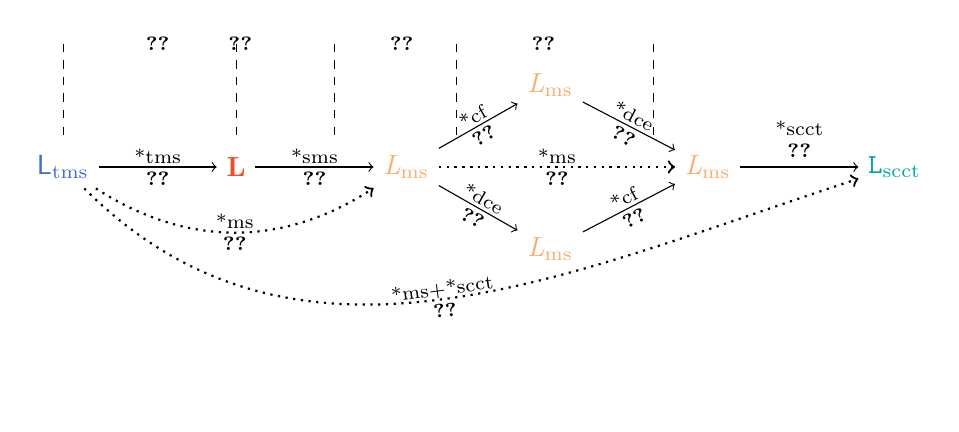
\begin{tikzpicture}
    \node (S) {$\src{L_{\tmssafe}}$};
    \node[right=1.5 of S] (T) {$\trg{L}$};
    \node[right=1.5 of T] (M) {$\irl{L_{\mssafe}}$};
    \node[below right=0.5 and 1.0 of M] (D0) {$\irl{L_{\mssafe}}$};
    \node[above right=0.5 and 1.0 of M] (C0) {$\irl{L_{\mssafe}}$};
    \node[right=3.0 of M] (E) {$\irl{L_{\mssafe}}$};
    \node[right=1.5 of E] (O) {$\obj{L_{\scctsafe}}$};

    \draw[->] (S) to[sloped] node[align=center,font=\scriptsize] (tmsedge) {\gls*{tms}\\ \Cref{thm:cca:rtp:tms}} (T);
    \draw[->] (T) to[sloped] node[align=center,font=\scriptsize] {\gls*{sms}\\ \Cref{thm:ccb:rtp:sms}} (M);
    \draw[->] (M) to[sloped] node[align=center,font=\scriptsize] {\gls*{dce}\\ \Cref{thm:ccdce:rtp:ms}} (D0);
    \draw[->] (M) to[sloped] node[align=center,font=\scriptsize] {\gls*{cf}\\ \Cref{thm:cccf:rtp:ms}} (C0);
    \draw[->] (D0) to[sloped] node[align=center,font=\scriptsize] {\gls*{cf}\\ \Cref{thm:cccf:rtp:ms}} (E);
    \draw[->] (C0) to[sloped] node[align=center,font=\scriptsize] {\gls*{dce}\\ \Cref{thm:ccdce:rtp:ms}} (E);
    \draw[->] (E) to[sloped,above] node[align=center,font=\scriptsize] {\gls*{scct}\\ \Cref{thm:ccscct:rtp:scct}} (O);

    % Sections
    \node[above=1.0 of tmsedge] (sectms) {{\scriptsize\Cref{subsec:cs:tms}}};
    \node[right=0.5 of sectms] (secsms) {{\scriptsize\Cref{subsec:cs:ms}}};
    \node[right=1.5 of secsms] (secopts) {{\scriptsize\Cref{subsec:cs:opts}}};
    \node[right=1.25 of secopts] (secscct) {{\scriptsize\Cref{subsec:cs:scct}}};

    \draw[thick,dotted,->] (S) to[bend right=33,sloped] node[align=center,font=\scriptsize] {\gls*{ms}\\ \Cref{thm:ccab:rtp:ms}} (M);
    \draw[thick,dotted,->] (M) to[bend right=0,sloped] node[align=center,font=\scriptsize] {\gls*{ms}\\ \Cref{thm:cccfccdce:rtp:ms}} (E);
    \draw[thick,dotted,->] (S) to[out=-45,in=198,sloped] node[align=center,font=\scriptsize] {\gls*{ms}+\gls*{scct}\\ \Cref{thm:ccall:rtp:msscct}} (O);

    \draw[dashed] ($(sectms)-(1.2,0)$) -- ($(sectms)-(1.2,1.25)$);
    \draw[dashed] ($(sectms)-(-1.0,0)$) -- ($(sectms)-(-1.0,1.25)$);
    \draw[dashed] ($(secsms)-(-1.2,0)$) -- ($(secsms)-(-1.2,1.25)$);
    \draw[dashed] ($(secscct)-(1.1,0)$) -- ($(secscct)-(1.1,1.25)$);
    \draw[dashed] ($(secscct)-(-1.4,0)$) -- ($(secscct)-(-1.4,1.25)$);
  \end{tikzpicture}
  % \vspace{-2.5em}
  \caption{Visualisation of the optimising compilation pipeline that attains a combination of \gls*{ms} and \gls*{cct}. %
    Vertices in the graph are the programming languages from earlier sections (\Cref{sec:casestud:defs}). %
    All edges are secure compilers, but dotted edges use the presented framework (\Cref{sec:compcomp}) and solid edges classic proof techniques. %
    The dashed lines partition the graph into the sections where the respective theorems are presented.
  }\label{fig:pipeline}
\end{figure*}
The section demonstrates the power of the framework (\Cref{sec:compprop,sec:compcomp}) by composing these compilers for a secure and optimising compilation chain that robustly preserves \gls*{msscct}.
The first step in this chain is the compiler from $\src{L_{\tmssafe}}$ to $\trg{L}$ that robustly preserves just \gls*{tms} (\Cref{thm:cca:rtp:tms}).
From here, an instrumentation from $\trg{L}$ to $\irl{L_{\mssafe}}$ ensures that no out-of-bounds accesses can happen and, thus, programs at this point attain \gls*{sms} (\Cref{thm:ccb:rtp:sms}).
Since these properties compose into \gls*{ms}, composing these passes yields a compiler that robustly preserves \gls*{ms} (\Cref{thm:ccab:rtp:ms}).
Then, the section presents two optimising translations, namely \gls*{cf} and \gls*{dce}, each of which robustly preserves \gls*{ms} (\Cref{thm:ccdce:rtp:ms,thm:cccf:rtp:ms}).
These translations can be freely ordered in the compilation chain without compromising memory safety (\Cref{thm:cccfccdce:rtp:ms}).
The last step of the chain ensures that code stays \gls*{scct} (\Cref{thm:ccscct:rtp:scct}) when lowered from $\Lms$ to $\Lscct$.
The final result is that the whole compilation chain robustly preserves \gls*{msscct} (\Cref{thm:ccall:rtp:msscct}).


\subsection{Robust Temporal Memory Safety Preservation}\label{subsec:cs:tms}

This subsection defines a secure compiler from $\Ltms$ to $\Ltrg$.
To this end, the compiler needs to ensure that when execution switches from context to component, the type signatures are respected.
It can do so by inserting dynamic typechecks prior to entering the body of a function belonging to the component.

\begin{gather*}
% \small
  \begin{aligned}
    \cca(\src{x}) = &\ \trg{x} 
    % \\
  	&
  	\qquad
    \cca(\src{\lbinop{\expr[_{1}]}{\expr[_{2}]}}) = &\ \lbinop[\trg]{\left[\cca(\src{\expr[_{1}]})\right]}{\left[\cca(\src{\expr[_{2}]})\right]} \\
    \cca(\src{n}) = &\ \trg{n} 
    % \\
    &
    \qquad
    \cca(\src{\lget{x}{\expr}}) = &\ \lget[\trg]{\trg{x}}{\left[\cca(\src{\expr})\right]}
  \end{aligned}
    \\
  \begin{aligned}
    \cca(\src{\ldelete{x}}) = &\ \ldelete[\trg]{\left[\cca(\src{x})\right]} \\
%    \cca(\src{\lset{x}{\expr[_{1}]}{\expr[_{2}]}}) & = \lset[\trg]{\left[\cca(\src{x})\right]}{\left[\cca(\src{\expr[_{1}]})\right]}{\left[\cca(\src{\expr_{2}})\right]} \\
\cca(\src{\lfunction{g}{x:\natt\to\type[_{e}]}{\expr}})  = &\ \lfunction[\trg]{\trg{g}}{\trg{x}}{\lifz[\trg]{\trg{\lhast{x}{\natt}}}{
\\%
                                                            &
                                                            \left[\cca(\src{\expr})\right] %
                                                                                                 }{\labort[\trg]}}
  \end{aligned}
\end{gather*}

Since $\trg{L}$ has no static typechecks, it could happen that a bogus context $\trg{\library_{\ctx}}$ invokes a callable object accepting a $\src{\natt}$ with $\trg{\lpair{17}{29}}$.
By inserting the check, the compiler ensures that execution does not proceed in such cases.
The compiler does not insert other checks and proceeds as the identity function (which in this paper amounts to a simple re-colouring of $\src{L_{\tmssafe}}$ to $\trg{L}$ expressions).

Compiling the \texttt{strncpy} function from \Cref{sec:introduction} with $\cca$, the compiler would in this case ensure that the arguments that are evaluated in the compiled \texttt{strncpy} are valid.
% \MP{put the proof section in an appendix}

\begin{theorem}[$\cca$ is secure with respect to \gls*{tms}]\label{thm:cca:rtp:tms}
  $\rtp{\cca}{\tmssafe}$ % \Coqed
\end{theorem}

% \subsubsection{Proving Robust Safety Property Preservation}

% We illustrate the proof of \Cref{thm:cca:rtp:tms} since the other secure compilation proofs of this paper follow the same approach.
% Unfolding the theorem statement yields the following assumptions:  
%   for any $\pi\in\lceil\tmssafe\rceil$\footnote{$\lceil\cdot\rceil$ lifts the property to a hyperproperty by applying the powerset operation~\cite{clarkson2008hyper}.}, 
%   $\src{\trace}$, 
%   $\src{\runtimetermvar}$, 
%   and component $\src{\library_{comp}}$, 
%   we have that $\rsat{\src{\library_{comp}}}{\pi}$ and 
%   $\progstepto{\prog[\trg]{\trg{\library_{\ctx}}}{\cca(\src{\library_{\comp}})}}{\trg{\runtimetermvar}}{\trg{\trace}}$, where $\trg{\library_{\ctx}}$ is arbitrary.
% The proof obligation is $\msfilterL{\trg{\trace}}\in\pi$, i.e., the specification trace associated to $\trg{\trace}$ satisfies the property $\pi$.
% A way to show this is to relate trace $\trg{\trace}$ to some $\Ltms$ trace $\src{\trace}$ (which already satisfies the property as per the assumptions).
% The assumptions already contain a target execution associated to this trace, so the task is to find an associated $\Ltms$ execution that yields $\trg{\trace}$.
% The trace $\trg{\trace}$ is split into different parts, as commonly done in secure compilation works~\cite{korashy2021capableptrs,abate2018goodcomps}, where each part contains the events that either the context or the component does, but not both.
% Because of this, all such trace segments are ,,well-bracketed'' in the sense that they start with either $\trg{\ev{Start}}$, $\trg{\ev{Call}\ \comptoctx\ foo\ \valueexpr}$, or $\trg{\ev{Ret}\ \comptoctx\ \valueexpr}$ and end with either $\trg{\ev{End}\ \valueexpr}$, $\trg{\ev{Ret}\ \ctxtocomp\ \valueexpr}$, or $\trg{\ev{Call}\ \ctxtocomp\ foo\ \valueexpr}$.
% In the following, the former is referred to as a context segment, since these executions happen in $\trg{\library_{\ctx}}$, and the latter is referred to as a component segment, since these executions happen in $\cca(\src{\library_{\comp}})$.
% \Cref{fig:proofdiag:rtp} visualises this division for a program execution with one call from context to component and how the target execution is related to a source execution.
% In the figure, the green dashed lines encompass the component segments while the orange boxes contain the actual context switches from context to component or vice versa.
% From a technical perspective, as typically done in compilation proofs, the proof requires some setup to maintain a relation between $\src{\Omega}$ and $\trg{\Omega}$ .
% Two cross-language relations make this precise: (i) $\multimap_{\delta}$ relates states that are involved in a context segment, allowing the target execution to perform internal calls, and (ii) $\approx_{\delta}$ relates states that are involved in a component segment, where both states need to agree exactly, i.e., the memory and the control flow states are required to contain the same information.
% The relations are indexed with $\delta$, which is an injective mapping from $\Ltms$ locations $\src{\loc}$ to $\Ltrg$ locations $\trg{\loc}$.
% %Note that the relations $\multimap_{\delta}$ and $\approx_{\delta}$ swap when context switching.

% So far, the paper explained how to relate an $\Ltms$ execution with a $\Ltrg$ execution.
% The next question is therefore how to build the corresponding $\Ltms$ execution.
% This is done using a standard secure compilation proof technique called trace-based backtranslation~\cite{abate2019jour,korashy2021capableptrs,patrignani2021rsc}, which can be used to build a context $\src{\library_{\ctx}}$ that behaves similar to $\trg{\library_{\ctx}}$.
% % Since $\Ltms$ is statically typed, the context $\src{\library_{\ctx}}$ obtained from the backtranslation needs to be well-typed when linked with $\src{\library_{\comp}}$.
% For context segments of the trace $\trg{\trace}$ it is also necessary to show that the execution behaves similarily, i.e., the context obtained from the backtranslation generates trace $\src{\trace}$.
% For component segments of the trace, the relatedness of states and traces follows from a compiler correctness argument.
% These two arguments yield the source execution $\progstepto{\src{\prog{\library_{\ctx}}{\library_{\comp}}}}{\src{\runtimetermvar}}{\src{\trace}}$.

% The proof now works as follows.
% Given that $\msfilterL{\trg{\trace}}=\msfilterLtms{\src{\trace}}$, the proof goal changes from $\msfilterL{\trg{\trace}}\in\pi$ to $\msfilterLtms{\src{\trace}}\in\pi$.
% This follows by specializing the robust satisfaction assumption $\rsat{\src{\library_{\comp}}}{\pi}$ to use the context $\src{\library_{\ctx}}$, which is obtained from the backtranslation, and to use the source execution $\progstepto{\src{\prog{\library_{\ctx}}{\library_{\comp}}}}{\src{\runtimetermvar}}{\src{\trace}}$.

% \begin{figure*}[!ht]
%   \begin{center}
%     \begin{tikzpicture}[state/.style={minimum height=1.5cm}]
%       % relative horizontal/vertical distance between states
%       \pgfmathsetmacro{\hdist}{0.95}
%       \pgfmathsetmacro{\vdist}{1.35}
%       \pgfmathsetmacro{\halfvdist}{0.725}

%       % row of src states
%       \node[state] (srcempty) {$\rtt{\src{\emptyset}}{\src{\lcall{main}{0}}}$};
%       \foreach \s [remember=\s as \cur (initially empty)] in {1,w_1,p,w_2,2} {
%         \node[state,right=\hdist of src\cur] (src\s) {$\rtt{\src{\Omega_{\s}}}{\src{\expr[_{\s}]}}$};
%       }
%       % row of trg states
%       \node[state,below=\vdist of srcempty] (trgempty) {$\rtt{\trg{\emptyset}}{\trg{\lcall{main}{0}}}$};
%       \foreach \s in {1,w_1,p,w_2,2} {
%         \node[state,below=\vdist of src\s] (trg\s) {$\rtt{\trg{\Omega_{\s}}}{\trg{\expr[_{\s}]}}$};
%       }
%       %% illustrations
%         % backtrans wrapper 1
%         \draw[ultra thick,loosely dotted,Peach!50,rounded corners] (src1.north east) -- (srcw\string_1.north east)
%           -- (trgw\string_1.south east) -- (trg1.south west) -- (src1.north west) -- cycle;
%         % backtrans wrapper 2
%         \draw[ultra thick,loosely dotted,Peach!50,rounded corners] (srcp.north east) -- (srcw\string_2.north east)
%           -- (trgw\string_2.south east) -- (trgp.south west) -- (srcp.north west) -- cycle;
%         % compiler correctness
%         \draw[ultra thick,loosely dashed,Emerald!50,rounded corners] ($(srcw\string_1.north east)+(0,0.05)$) -- ($(srcp.north east)+(0,0.05)$)
%           -- ($(trgw\string_2.north east)+(0.05,0)$) -- ($(trgw\string_2.south east)+(0.05,-0.05)$)
%           -- ($(trg1.south west)+(-0.05,-0.05)$) -- ($(trg1.north west)+(-0.05,0)$) -- ($(srcw\string_1.north west)+(0,0.05)$) -- cycle;
%       % state relations
%       \path (srcempty) edge[very thick,draw=gray!25] node[pos=0.5,sloped,rotate=180,fill=white] {\scriptsize$\multimap_\emptyset$} (trgempty)
%         (src1) edge[very thick,draw=gray!25] node[pos=0.5,sloped,rotate=180,fill=white] {\scriptsize$\multimap_{\delta_1}$} (trg1)
%         (srcp) edge[very thick,draw=gray!25] node[pos=0.5,sloped,fill=white] {\scriptsize$\approx_{\delta_p}$} (trgp)
%         (src2) edge[very thick,draw=gray!25] node[pos=0.5,sloped,rotate=180,fill=white] {\scriptsize$\multimap_{\delta_2}$} (trg2)
%         (srcw\string_1) edge[very thick,draw=gray!25] node[pos=0.5,sloped,fill=white] {\scriptsize$\approx_{\delta_{w_1}}$} (trgw\string_1)
%         (srcw\string_2) edge[very thick,draw=gray!25] node[pos=0.5,sloped,rotate=180,fill=white] {\scriptsize$\multimap_{\delta_{w_2}}$} (trgw\string_2)
%         % diagonals
%         (srcw\string_1) edge[thick,draw=gray!25] node[pos=0.16,sloped,rotate=180,fill=white] {\scriptsize$\approx_{\delta_{w_1}}$} (trg1)
%         (src1) edge[thick,draw=gray!25] node[pos=0.16,sloped,rotate=180,fill=white] {\scriptsize$\multimap_{\delta_1}$} (trgw\string_1)
%         (srcp) edge[thick,draw=gray!25] node[pos=0.2,sloped,fill=white] {\scriptsize$\approx_{\delta_p}$} (trgw\string_2)
%         (trgp) edge[thick,draw=gray!25] node[pos=0.2,sloped,fill=white] {\scriptsize$\multimap_{\delta_{w_2}}$} (srcw\string_2)
%         ;
%       %\drawpolygon src1,srcw\string_1,trgw\string_1,trg1;
%       %\drawpolygon srcp,srcw\string_2,trgw\string_2,trgp;
%       %\node[font=\tiny,align=center,above=0.2 of srcw1srcp] (wrapper) {Backtranslation\\Wrapper};
%       %\path[->,draw] (wrapper) -- (srcw\string_1);
%       %\path[->,draw] (wrapper) -- (srcp);
%       % steps
%       \path[very thick,color=\stlccol] (srcempty) edge[draw=none] node {\ $\xrightarrow{\trace[_1]}{}{\kern-3.5pt}_{\text{ctx}}^*$} (src1)
%         (src1) edge[draw=none] node {\ $\xrightarrow{\trace[_c]}{}{\kern-3.5pt}_{\text{ctx}}$} (srcw\string_1)
%         (srcw\string_1) edge[draw=none] node {\ $\xrightarrow{\trace[_p]}{}{\kern-3.5pt}_{\text{ctx}}^*$} (srcp)
%         (srcp) edge[draw=none] node[fill=white,inner sep=0,outer sep=0] {\ $\xrightarrow{\trace[_r]}{}{\kern-3.5pt}_{\text{ctx}}$} (srcw\string_2)
%         (srcw\string_2) edge[draw=none] node {\ $\xrightarrow{\trace[_2]}{}{\kern-3.5pt}_{\text{ctx}}^*$} (src2)
%         ;
%       \path[very thick,color=\ulccol] (trgempty) edge[draw=none] node[fill=white,inner sep=0,outer sep=0] {\ $\xrightarrow{\phantom{\trace[_1]}}{}{\kern-3.5pt}_{\text{ctx}}^*$} (trg1)
%         (trg1) edge[draw=none] node {\ $\xrightarrow{\phantom{\trace[_p]}}{}{\kern-3.5pt}_{\text{ctx}}^*$} (trgw\string_1)
%         (trgw\string_1) edge[draw=none] node[fill=white,inner sep=0,outer sep=0] {\ $\xrightarrow{\phantom{\trace[_p]}}{}{\kern-3.5pt}_{\text{ctx}}^*$} (trgp)
%         (trgp) edge[very thick,draw=none] node {\ $\xrightarrow{\phantom{\trace[_p]}}{}{\kern-3.5pt}_{\text{ctx}}^*$} (trgw\string_2)
%         (trgw\string_2) edge[draw=none] node {\ $\xrightarrow{\phantom{\trace[_2]}}{}{\kern-3.5pt}_{\text{ctx}}^*$} (trg2)
%         ;
%       % legend
% %     \node[align=left,below right=0.3 and 0.3 of trgempty,font=\tiny] (legend) {%
% %       ${\src{\trace[_c]}}\cong{\backt{\Ltms}{\Ltrg}(\trg{Call\ ?\ foo\ \valueexpr})}$\\%
% %       ${\src{\trace[_r]}}\cong{\backt{\Ltms}{\Ltrg}(\trg{Ret\ !\ foo\ \valueexpr})}$
% %       };
%       \node[below=0.5 of trgempty,draw=none] (legend) {};
%       \draw[ultra thick,loosely dotted,Peach!50,rounded corners] ($(legend.north east)+(0.5,-0.4)$) -- ($(legend.north east)+(1,-0.4)$);
%       \node at ($(legend.north east)+(1.5,-0.4)$) (legendwrapper) {};
%       \node[right of=legendwrapper] {\tiny Backtranslation Wrapper};
%       \draw[ultra thick,loosely dashed,Emerald!50,rounded corners] ($(legend.south east)+(0.5,0.4)$) -- ($(legend.south east)+(1,0.4)$);
%       \node at ($(legend.south east)+(1.5,0.4)$) (legendcorrectness) {};
%       \node[right of=legendcorrectness] {\tiny Compiler Correctness};
%     \end{tikzpicture}
%     \caption{Proof diagram for \Cref{thm:cca:rtp:tms} depicting the general structure of robust preservation proofs. %
%       Nodes in the graph represent runtime states. %
%       Vertical lines indicate cross language relations, while horizontal ones are execution steps. %
%       The green dashed trapezoid encompasses the component segment, while the orange dotted rectangles entail the context switches. %
%       $\Ltrg$ traces are omitted for readability. %
%       $\Ltms$ trace segments $\src{\trace[_{c}]}$ and $\src{\trace[_{r}]}$ describe the events that happen at the boundaries, i.e., during a context switch.
%       $\src{\trace_{p}}$ is the behavior of the component and the traces $\src{\trace[_{1}]}$ and $\src{\trace[_{2}]}$ describe the context.
%     }\label{fig:proofdiag:rtp}
%   \end{center}
% \end{figure*}

% \MPpost{
% 	this can be made more precise
% }

\subsection{Robust Spatial Memory Safety Preservation}\label{subsec:cs:ms}

\vspace{-1em}
\begin{center}
% \small
  $$
  \begin{array}{rcl}
    \ccb(\trg{\lnew{x}{\expr[_{1}]}{\expr[_{2}]}}) & = 
                                                   & \llet[\irl]{\irl{x_{SIZE}}}{\ccb(\trg{\expr[_{1}]})}{}
    		\\&&
    		\lnew[\irl]{\irl{x}}{\irl{x_{SIZE}}}{\ccb(\trg{\expr[_{2}]})}
    		 \\
  \ccb(\trg{\lget{x}{\expr}}) & = 
                              & \llet[\irl]{\irl{x_{n}}}{\ccb(\trg{\expr})}{}
  	\\&&
  \lifz[\irl]{\irl{0\le x_{n}<x_{SIZE}}}{\\&&\irl{\lget{x}{x_{n}}}}{}
  		\irl{\labort}
  	  \\
  \ccb(\trg{\lset{x}{\expr[_{1}]}{\expr[_{2}]}}) & = 
                                                 & \llet[\irl]{\irl{x_{n}}}{\ccb(\trg{\expr[_{1}]})}{}
  		\\&&
  \lifz[\irl]{\irl{0\le x_{n}<x_{SIZE}}}{\\&&\lset[\irl]{\irl{x}}{\irl{x_{n}}}{}
  		\ccb(\trg{\expr[_{2}]})
  		}{\irl{\labort}} 
  		% \\
  \end{array}
  $$
\end{center}

The compiler $\cc{\trg{L}}{\Lms}$ only inserts bounds-checks whenever reading from or writing to memory in order to enforce \gls*{sms}.
For passing pointers, it has to pass them with their size information as well.
To this end, the compiler introduces another, fresh identifier $\irl{x_{SIZE}}$ for each allocation that binds $\irl{x}$ to keep track of the allocation size.
\begin{exampleenv}[Instrumented \texttt{strncpy}]
  Consider again \texttt{strncpy}, but instrumented for \gls*{sms}:
    \begin{lstlisting}[language=c,basicstyle=\ttfamily\footnotesize, morekeywords={size_t}]
void strncpy(size_t n, size_t dst_size, char *dst,
             size_t src_size, char *src) {
  for(size_t i = 0; i < src_size && src[i] != '\0' && i < n; ++i) {
    if(i < src_size && i < dst_size) {
      dst[i] = src[i];
    }
  }
}
    \end{lstlisting}
    When calling this with a context like in \Cref{ex:strncpy:sms}, the event $\ev{Use}\ \loc_{x}\ 2;\comp;\unlock$ would not be emitted during execution, since the bounds check prevents the condition \texttt{src[i] != '\textbackslash 0'} from executing.
\end{exampleenv}

\begin{theorem}[$\ccb$ is secure with respect to \gls*{sms}]\label{thm:ccb:rtp:sms}
  $\rtp{\ccb}{\smssafe}$ % \Coqed
\end{theorem}

\Cref{thm:ccab:rtp:ms} states that the composition of $\cca$ and $\ccb$ is secure with respect to \gls*{ms} and follows from \Cref{thm:cca:rtp:tms,thm:ccb:rtp:sms} using \Cref{thm:rtp}.

\begin{theorem}[$\cca\circ\ccb$ is secure with respect to \gls*{ms}]\label{thm:ccab:rtp:ms}
  $\rtp{\cca\circ\ccb}{\mssafe}$ % \Coqed
\end{theorem}
% \begin{proof}\MP{keep?}
%   From \Thmref{thm:cca:rtp:tms} it follows that for any $\Ltms$ program $\src{\progvar}$, it compiles to an $\Ltrg$ program $\trg{\progvar}$ that robustly satisfies \gls*{tms}.
%   Note that $\src{\progvar}$ robustly satisfies \gls*{tms} by the properties of the typesystem of $\Ltms$.
%   Then, \Thmref{thm:ccb:rtp:sms} demonstrates that, assuming $\trg{\progvar}$ robustly satisfies \gls*{sms}, the program $\trg{\progvar}$ compiles to an $\Lms$ program $\irl{p}$ that also robustly satisfies \gls*{sms}.
%   From \Thmref{thm:ccab:rtp:ms} it follows that $\src{p}$ compiles to $\irl{p}$ that robustly satisfies \gls*{ms}, since \gls*{ms} is the intersection of \gls*{tms} and \gls*{sms}.
% \end{proof}

\subsection{Optimising Compilers}\label{subsec:cs:opts}

\vspace{-1em}
\begin{gather*}
  \begin{align*}
    \ccdce(\irl{\lifz{true}{\expr[_{1}]}{\expr[_{2}]}}) & = \ccdce(\irl{\expr[_{1}]}) &\\
    \ccdce(\irl{\lifz{false}{\expr[_{1}]}{\expr[_{2}]}}) & = \ccdce(\irl{\expr[_{2}]}) &
  \end{align*}
  \\
  % \begin{align*}
  %   \ccdce(\irl{\lbinop{\expr[_{1}]}{\expr[_{2}]}}) & = \lbinop[\irl]{\ccdce(\irl{\expr[_{1}]})}{\ccdce(\irl{\expr[_{2}]})} &
  % \end{align*}
  % \\[0.25cm]
  \begin{align*}
    \cccf(\irl{\expr}) & = \partialeval{\irl{\expr}}{\irl{\hole{\cdot}}} &
  \end{align*}
  \\[0.125cm]
  \begin{align*}
   \partialeval{\irl{x}}{\irl{\substlist}} & = \irl{n} 
   	\qquad\qquad \text{if } \irl{\subst{n}{x}}\in\irl{\substlist} \\
   \partialeval{\irl{x}}{\irl{\substlist}} & = \irl{x} 
   \qquad\qquad \text{if } \irl{\subst{n}{x}}\notin\irl{\substlist} \\
   \partialeval{\irl{\lbinop{n}{m}}}{\irl{\substlist}} & = \irl{k} 
   \qquad\qquad \text{if } \lbinop{\irl{n}}{\irl{m}}=k \\
   %\partialeval{\irl{\lbinop{\expr[_{1}]}{\expr[_{2}]}}}{\irl{\substlist}} & = \lbinop[\irl]{\partialeval{\irl{\expr[_{1}]}}{\irl{\substlist}}}{\partialeval{\irl{\expr[_{2}]}}{\irl{\substlist}}} \\
   \partialeval{\irl{\llet{x}{\valueexpr}{\expr}}}{\irl{\substlist}} & = \partialeval{\irl{\expr}}{\irl{\subst{x}{\valueexpr}\cdot\substlist}} 
  % \\
  % \partialeval{\irl{\lget{x}{\expr}}}{\irl{\substlist}} & = \lget[\irl]{\irl{x}}{\partialeval{\irl{\expr}}{\irl{\substlist}}}
% \end{align*}
\end{align*}
% \\
% \begin{align*}
%   \partialeval{\irl{\llet{x}{\expr[_{1}]}{\expr[_{2}]}}}{\irl{\substlist}} & = \llet[\irl]{\irl{x}}{\partialeval{\irl{\expr[_{1}]}}{\irl{\substlist}}}{\\&\partialeval{\irl{\expr[_{2}]}}{\irl{\substlist}}} \\
%   \partialeval{\irl{\lifz{\expr[_{1}]}{\expr[_{2}]}{\expr[_{3}]}}}{\irl{\substlist}} & = \lifz[\irl]{\partialeval{\irl{\expr[_{1}]}}{\irl{\substlist}}}{\\&\partialeval{\irl{\expr[_{2}]}}{\irl{\substlist}}}{\partialeval{\irl{\expr[_{3}]}}{\irl{\substlist}}} \\
% \end{align*}
\end{gather*}
% \vspace{-3em}

The two optimising compiler passes from $\Lms$ to $\Lms$ perform \gls*{dce} and \gls*{cf}, respectively.
The \gls*{dce} pass applies a naive rewrite rule on conditionals.
The \gls*{cf} pass relies on an auxiliary function \texttt{mix} that uses a substitutions accumulator $\irl{\substlist}$ in order to rewrite constant binary operations, e.g., $\irl{{17}-1}$ to $\irl{16}$, and replace variables that are assigned to constants with their constant, e.g., $\irl{\llet{x}{7}{x}}$ to $\irl{7}$.
Both passes are secure with respect to \gls*{ms}.
The proof for either is relatively simple, because both \gls*{dce} and \gls*{cf} do not change the way memory accesses happen.
Moreover, since the input and output languages to these compilers are the same, attacker contexts do not have more power in the target language than in the source, since both languages are equal.

\begin{theorem}[$\ccdce$ is secure with respect to \gls*{ms}]\label{thm:ccdce:rtp:ms}
  $\rtp{\ccdce}{\mssafe}$ %\Coqed
\end{theorem}
\begin{theorem}[$\cccf$ is secure with respect to \gls*{ms}]\label{thm:cccf:rtp:ms}
  $\rtp{\cccf}{\mssafe}$ %\Coqe
\end{theorem}

With both \Cref{thm:ccdce:rtp:ms,thm:cccf:rtp:ms} it follows from \Cref{corr:swappable} that the two passes can be interchanged arbitrarily:

\begin{theorem}[$\cccf\circ\ccdce$ and $\cccf\circ\ccdce$ are secure with respect to \gls*{ms}]\label{thm:cccfccdce:rtp:ms}
  $\rtp{\cccf\circ\ccdce}{\mssafe}$ and $\rtp{\ccdce\circ\cccf}{\mssafe}$. % \Coqed
\end{theorem}

\subsection{Robust Strict Cryptographic Constant Time Preservation}\label{subsec:cs:scct}

\vspace{-1em}
\begin{center}\small
  \begin{align*}
    \ccscct(\irl{\lfunction{g}{x}{\expr}}) & = \lfunction[\obj]{\obj{g}}{\obj{x}}{\obj{\lwrdoit{ON};}\ccscct(\irl{\expr})} \\
    \ccscct(\irl{\lcall{g}{\expr}}) & = \lcall[\obj]{\obj{g}}{\ccscct(\irl{\expr})\obj{; \lwrdoit{ON}}} 
    % \\
    % \ccscct(\irl{\lbinop{\expr[_{1}]}{\expr[_{2}]}}) & = \lbinop[\obj]{\ccscct{\irl{\expr[_{1}]}}}{\ccscct{\irl{\expr[_{2}]}}} 
    % \\
  \end{align*}
\end{center}
% \vspace{-2em}
%
Given the fact that $\Lscct$ provides a \gls*{cct}-mode that can be turned on or off, the compiler inserts wrapper code for function bodies to ensure that execution in the component always happen in this \gls*{cct}-mode.
The context can overwrite the flag and exit the mode, but upon invoking a function that is part of the component, the flag would be set again.
Because of this, the compiler is secure with respect to \gls*{scct}, similarly proven as in \Cref{subsec:cs:tms}.

\begin{theorem}[$\ccscct$ is secure with respect to \gls*{scct}]\label{thm:ccscct:rtp:scct}
  $\rtp{\ccscct}{\scctsafe}$ % \Coqed
\end{theorem}

\subsection{Robust Preservation of Intersection of Memory Safety and Strict Cryptographic Constant Time}

Let $\ccmsscct$ be the compiler that is the composition of $\cca$, $\ccb$, $\cccf$, $\ccdce$, and $\ccscct$, then the following theorem holds.

\begin{theorem}[$\ccmsscct$ is secure with respect to \gls*{scct}]\label{thm:ccall:rtp:msscct}
  $\rtp{\cc{\Ltms}{\Lscct}}{\mssafe\cap\scctsafe}$ % \Coqed
\end{theorem}
% \begin{proof}\MP{keep?}
% 	From \Thmref{thm:ccab:rtp:ms}, we have that any $\Ltms$ program $\src{\progvar}$ compiles into a $\Lms$ program $\irl{\progvar}$ that robustly satisfies \gls*{ms}.
% 	Then, from \Thmref{thm:cccfccdce:rtp:ms} we have that $\irl{\progvar}$ gets optimised to a program $\irl{\progvar[']}$ that is also \gls*{ms}, where the order of optimisations does not matter for $\irl{\progvar[']}$ to be \gls*{ms}.
%   Assuming $\irl{\progvar[']}$ robustly satisfies \gls*{scct}, by \Thmref{thm:ccscct:rtp:scct} it compiles to an $\Lscct$ program $\obj{\progvar}$ that robustly satisfies \gls*{scct} as well.
%   Finally, from \Thmref{thm:rtp} it follows that, given $\src{\progvar}$ robustly satisfies \gls*{scct} and \gls*{ms}, $\obj{\progvar}$ also robustly satisfies \gls*{scct} and \gls*{ms}.
% \end{proof}

\subsection{Robust Speculative Safety Preservation}\label{subsec:cs:ss}

\vspace{-1em}
\begin{center}\small
  \begin{align*}
    \ccspec(\obj{\lifz{\expr[_0]}{\expr[_1]}{\expr[_2]}}) & = \lifz[\ird]{\ccspec{\left(\obj{\expr[_0]}\right)}}{\\&\ird{\lbarrier;}\ccspec{\left(\obj{\expr[_1]}\right)}\\&}{\ird{\lbarrier;}\ccspec{\left(\ird{\expr[_2]}\right)}} \\
  \end{align*}
\end{center}
% \vspace{-2em}
%
\begin{theorem}[$\ccspec$ is secure with respect to \gls*{ss}]\label{thm:ccspec:rtp:spec}
  $\rtp{\ccspec}{\specmssafe}$ % \Coqed
\end{theorem}

\section{Related Work\pages{2}}\label{sec:relwork}

This section discusses work on robust compilation (\Cref{subsec:relw:seccomprtp}) and on other secure compilation criteria (\Cref{subsec:relw:seccompcrit}).
Since the case study of \Cref{sec:casestud:defs,sec:casestud:rtp} implements measures for preserving \gls*{ms} and \gls*{cct}, this section then presents relevant related work as well (\Cref{subsec:relw:msmechs,subsec:relw:cctmechs}).

\subsection{Secure Compilation as Robust Preservation}\label{subsec:relw:seccomprtp}

The robust preservation of properties as a compiler-level criterion has been analyzed extensively~\cite{abate2019jour,patrignani2021rsc,abate2021extacc,patrignani2019survey} and thus we build on that framework.
No existing work is concerned with composing robustly safe compilers.
These works consider languages with different trace models and our technical setup can be adapted to that as long as security properties and their monitors are still defined on the same trace model.
The work relating robust preservation with universal composability~\cite{patrignani2022universal} is closest to what this paper presents.
The authors demonstrate a similar compositionality theorem to what is presented here (\Cref{sec:compcomp}) but use it in the context of protocols.
They do not demonstrate the scalability of the approach.
Moreover, they are missing the upper and lower compositions.
% The authors demonstrate a similar compositionality theorem to what is presented here (\Cref{sec:compcomp}) as well as in an earlier version of this work~\cite{kruse2022csc}.
% However, they do not demonstrate the scalability of the approach by means of a case study.

\subsection{Other Secure Compilation Criteria}\label{subsec:relw:seccompcrit}

While this paper focuses on the robust preservation framework~\cite{abate2019jour}, other secure compilation criteria exist.
The survey on formal approaches to secure compilation~\cite{patrignani2019survey} discusses a broad spectrum already, while this section presents a very high-level overview.
Fully abstract compilation~\cite{abadi1999fullabstraction} states that a compiler should preserve and reflect observational equivalence between source and target programs.
It was shown~\cite{abate2021faandrc} that fully abstract compilers robustly preserve program properties that are either trivial or meaningless.
As a mitigation for this, the authors presented a categorical approach based on maps of distributive laws~\cite{watanabe2002modl}, which they call many maps of distributive laws.
Maps of distributive laws have been investigated before as a possible secure compilation criterion~\cite{tsampas2020catsc}.
Other approaches are extensions of the compiler correctness criterion as discussed in other work~\cite{patterson2019next700} or the introduction of opaque observations~\cite{vu2021reconciling} to reconcile compiler optimisations with security.
Note that this work also presents secure compilers that are optimising, but contrary to the other~\cite{vu2021reconciling}, provides a formal account of these in the robust preservation framework.
% Lastly, the authors of this paper have presented ongoing work~\cite{patrignani2023blame} on a weaker robust preservation criteria based on the concept blame.

\subsection{Memory Safety Mechanisms}\label{subsec:relw:msmechs}

Different mechanisms for enforcing memory safety exist that also consider the secure compilation domain, i.e., have an active attacker model.
For example, the ,,pointers as capabilities'' principle represents pointers as machine-level capabilities~\cite{korashy2021capableptrs}, which behave in a similar fashion to capabilities by means of linear typing~\cite{morrisett2005L3}.
The approach of this paper also uses linear typing, but differs from $L^{3}$~\cite{morrisett2005L3} in the way that functions are not first-class.
Moreover, this paper considers an active attacker, while the work on $L^{3}$ only discusses whole programs and, thus, has no active attacker model.
The instrumentation to ensure memory safety that this paper presents is inspired by Softbounds~\cite{nagarakatte2009soft}.
That work inserts bounds-checks in front of pointer-dereferences and, for this to work, inserts meta-data information on pointer creation.
Softbounds also works in a more advanced setting with structured fields accesses and also introduces a table-lookup for pointers that are stored in memory.
This paper only considers arrays of primitive data, i.e., there are no pointers to pointers or structures.
Several other approaches to memory-safety exist in literature, specifically as compiler instrumentations~\cite{akritidis2009baggy,younan2010paricheck,jung2021pico,shankaranarayana2023tailcheck,dhumbumroong2020boundwarden,nam2019framer,zhou2023fatptrs}, hardware-extensions~\cite{kwon2013lowfat,saileshwar2022heapcheck,chen2023flexpointer,kim2023whistle}, or programming language extensions~\cite{elliott2018checkedc,li2022formalcheckedc,jim2002cyclone,elliott2015guilt,west2005cuckoo,weis2019fyr,benoit2019uniqueness}.
What differentiates this work from them is that this work uses known, compiler-based approaches to ensure memory-safety as a means to investigate secure compiler compositions.
This paper does not provide efficient memory-safety, but serves as a theoretical foundation for the secure compilation domain.

To extend the languages in this paper with a less restricted form of pointer arithmetic, the region coloring memory safety monitor presented in earlier work~\cite{michael2023mswasm} can be used.
The work presenting this monitor provides an approach for the robust preservation of memory safety compiling from C to WASM.
However, they do not discuss composition of secure compilers but rather investigate an instance of a secure compiler.

\subsection{Cryptographic Constant Time Mechanisms}\label{subsec:relw:cctmechs}

The approach to preserving cryptographic constant time in this paper is high-level, where a programming language exposes a way to switch the semantics to a data (operand) independent timing mode.
Since identifiers in $\Lscct$ are annotated with a secrecy tag, this approach is similar to others with information flow control.
For example, Vale~\cite{bond2017vale} uses Dafny to ensure constant-time assembly code, while Jasmin~\cite{almeida2017jasmin} makes use of the Coq proof assistant to reject non-constant-time programs.
CT-Wasm~\cite{watt2019ctwasm} enforces constant-timeness by means of a type system.
Different to the approach of this paper, these approaches necessitate that the programmer writes \gls*{cct} code.
An approach to allow programmers to write more high-level code is CryptOpt~\cite{kuepper2023cryptopt}, which generates efficient target-code by means of a randomised search.
This paper abstracts over concrete mitigation strategies and simply assumes that there is a flag to switch to a cryptographic-constant time execution mode.
This can be realised by employing the FaCT~\cite{cauligi2019fact} compiler, which translates common non-constant time code patterns to be constant-time, and the data (object) independent timing execution mode of modern processors.

\section{Conclusion\pages{$\sfrac{1}{2}$}}\label{sec:concl}
This paper tackled the problem of understanding what kind of security properties does a secure compiler preserve, when said compiler is the combination of compiler passes that preserve possibly different security properties.
% 
For this, this paper first formalised security properties of interest and their composition.
% 
Then, it proved that composing secure compilers that preserve certain properties results in a secure compiler that preserves the composition of these properties.
% While the presented security property composition relied on monitors that check only trace-properties, the composition of secure compilers does not make any restriction towards the kind of property involved in the composition. 
% It is subject to future work to develop techniques to verify relational hyperproperties~\cite{abate2019jour}, while the composition of hyperproperties could be very similar to the composition of ordinary properties as presented in this paper, since hyperproperties can be checked with an automata-based model-checker~\cite{beutner23hyperltl}.
% 
Finally, this paper defines a multi-pass compiler and proves that it preserves \gls*{msscct}.
Crucially, this paper derives the security of the multi-pass compiler from the composition of the security properties preserved by its individual passes, which include security-preserving as well as optimisation passes.
% For future work, it is interesting to look at more sophisticated optimisation passes that, e.g., reorder events that appear on traces.


% This paper does a first step towards practical secure compilation chains by introducing a theoretical framework demonstrating that secure compilers compose.
% The paper exercises this framework on a case-study that consists of an optimising compilation chain that is secure with respect to \gls*{msscct}.
% \MP{
% 	not an appropriate recap.
% 	rewrite summarising the paper
% }

% In future work, it would be interesting to investigate whether it is possible to provide {\em secure compiler combinators}, similarly to how parser combinators work.
% %To this end, it may be necessary to extend existing frameworks for multi-language semantics.
% It is also interesting to extend our case-study and verify all results of it in Coq.
% This way, it is possible to obtain an executable, secure compiler.
% However, the formalisation effort for backtranslation proofs is known to be enormous\MP{cit + details}, so another research avenue may be to find better ways to (semi-)automate standard secure compilation proofs.
% \MPin{
% 	not particularly informative FW. i'd rather not have it as such
% }

%% The acknowledgments section is defined using the "acks" environment
%% (and NOT an unnumbered section). This ensures the proper
%% identification of the section in the article metadata, and the
%% consistent spelling of the heading.

% \begin{acks}
%   We would like to thank the anonymous reviewers for their feedback.
% 	This work was partially supported by a gift from
		% the Italian Ministry of Education through funding for the Rita Levi Montalcini grant (call of 2019).
% \end{acks}

% \section*{Acknowledgements}\label{sec:acks}

% \section*{Appendix}

% The appendix contains insights on the structure of proofs for the theorems of \Cref{sec:casestud:rtp} (\Cref{sec:proof-sketch}).
% Then it contains the proof of \Thmref{thm:ccab:rtp:ms} (\Cref{sec:proof1}) and of \Thmref{thm:ccall:rtp:msscct} (\Cref{sec:proof2}).

% \section{Proving Robust Safety Property Preservation}\label{sec:proof-sketch}

% We illustrate the proof of \Cref{thm:cca:rtp:tms} since the other secure compilation proofs of this paper follow the same approach.
% Unfolding the theorem statement yields the following assumptions:  
%   for any $\pi\in\lceil\tmssafe\rceil$\footnote{$\lceil\cdot\rceil$ lifts the property to a hyperproperty by applying the powerset operation~\cite{clarkson2008hyper}.}, 
%   $\src{\trace}$, 
%   $\src{\runtimetermvar}$, 
%   and component $\src{\library_{comp}}$, 
%   we have that $\rsat{\src{\library_{comp}}}{\pi}$ and 
%   $\progstepto{\prog[\trg]{\trg{\library_{\ctx}}}{\cca(\src{\library_{\comp}})}}{\trg{\runtimetermvar}}{\trg{\trace}}$, where $\trg{\library_{\ctx}}$ is arbitrary.
% The proof obligation is $\msfilterL{\trg{\trace}}\in\pi$, i.e., the specification trace associated to $\trg{\trace}$ satisfies the property $\pi$.
% A way to show this is to relate trace $\trg{\trace}$ to some $\Ltms$ trace $\src{\trace}$ (which already satisfies the property as per the assumptions).
% The assumptions already contain a target execution associated to this trace, so the task is to find an associated $\Ltms$ execution that yields $\trg{\trace}$.
% The trace $\trg{\trace}$ is split into different parts, as commonly done in secure compilation works~\cite{korashy2021capableptrs,abate2018goodcomps}, where each part contains the events that either the context or the component does, but not both.
% Because of this, all such trace segments are ,,well-bracketed'' in the sense that they start with either $\trg{\ev{Start}}$, $\trg{\ev{Call}\ \comptoctx\ foo\ \valueexpr}$, or $\trg{\ev{Ret}\ \comptoctx\ \valueexpr}$ and end with either $\trg{\ev{End}\ \valueexpr}$, $\trg{\ev{Ret}\ \ctxtocomp\ \valueexpr}$, or $\trg{\ev{Call}\ \ctxtocomp\ foo\ \valueexpr}$.
% In the following, the former is referred to as a context segment, since these executions happen in $\trg{\library_{\ctx}}$, and the latter is referred to as a component segment, since these executions happen in $\cca(\src{\library_{\comp}})$.
% \Cref{fig:proofdiag:rtp} visualises this division for a program execution with one call from context to component and how the target execution is related to a source execution.
% In the figure, the green dashed lines encompass the component segments while the orange boxes contain the actual context switches from context to component or vice versa.
% From a technical perspective, as typically done in compilation proofs, the proof requires some setup to maintain a relation between $\src{\Omega}$ and $\trg{\Omega}$ .
% Two cross-language relations make this precise: (i) $\multimap_{\delta}$ relates states that are involved in a context segment, allowing the target execution to perform internal calls, and (ii) $\approx_{\delta}$ relates states that are involved in a component segment, where both states need to agree exactly, i.e., the memory and the control flow states are required to contain the same information.
% The relations are indexed with $\delta$, which is an injective mapping from $\Ltms$ locations $\src{\loc}$ to $\Ltrg$ locations $\trg{\loc}$.
% %Note that the relations $\multimap_{\delta}$ and $\approx_{\delta}$ swap when context switching.

% So far, the paper explained how to relate an $\Ltms$ execution with a $\Ltrg$ execution.
% The next question is therefore how to build the corresponding $\Ltms$ execution.
% This is done using a standard secure compilation proof technique called trace-based backtranslation~\cite{abate2019jour,korashy2021capableptrs,patrignani2021rsc}, which can be used to build a context $\src{\library_{\ctx}}$ that behaves similar to $\trg{\library_{\ctx}}$.
% % Since $\Ltms$ is statically typed, the context $\src{\library_{\ctx}}$ obtained from the backtranslation needs to be well-typed when linked with $\src{\library_{\comp}}$.
% For context segments of the trace $\trg{\trace}$ it is also necessary to show that the execution behaves similarily, i.e., the context obtained from the backtranslation generates trace $\src{\trace}$.
% For component segments of the trace, the relatedness of states and traces follows from a compiler correctness argument.
% These two arguments yield the source execution $\progstepto{\src{\prog{\library_{\ctx}}{\library_{\comp}}}}{\src{\runtimetermvar}}{\src{\trace}}$.

% The proof now works as follows.
% Given that $\msfilterL{\trg{\trace}}=\msfilterLtms{\src{\trace}}$, the proof goal changes from $\msfilterL{\trg{\trace}}\in\pi$ to $\msfilterLtms{\src{\trace}}\in\pi$.
% This follows by specializing the robust satisfaction assumption $\rsat{\src{\library_{\comp}}}{\pi}$ to use the context $\src{\library_{\ctx}}$, which is obtained from the backtranslation, and to use the source execution $\progstepto{\src{\prog{\library_{\ctx}}{\library_{\comp}}}}{\src{\runtimetermvar}}{\src{\trace}}$.

% \begin{figure*}[!ht]
%   \begin{center}
%     \begin{tikzpicture}[state/.style={minimum height=1.5cm}]
%       % relative horizontal/vertical distance between states
%       \pgfmathsetmacro{\hdist}{0.95}
%       \pgfmathsetmacro{\vdist}{1.35}
%       \pgfmathsetmacro{\halfvdist}{0.725}

%       % row of src states
%       \node[state] (srcempty) {$\rtt{\src{\emptyset}}{\src{\lcall{main}{0}}}$};
%       \foreach \s [remember=\s as \cur (initially empty)] in {1,w_1,p,w_2,2} {
%         \node[state,right=\hdist of src\cur] (src\s) {$\rtt{\src{\Omega_{\s}}}{\src{\expr[_{\s}]}}$};
%       }
%       % row of trg states
%       \node[state,below=\vdist of srcempty] (trgempty) {$\rtt{\trg{\emptyset}}{\trg{\lcall{main}{0}}}$};
%       \foreach \s in {1,w_1,p,w_2,2} {
%         \node[state,below=\vdist of src\s] (trg\s) {$\rtt{\trg{\Omega_{\s}}}{\trg{\expr[_{\s}]}}$};
%       }
%       %% illustrations
%         % backtrans wrapper 1
%         \draw[ultra thick,loosely dotted,Peach!50,rounded corners] (src1.north east) -- (srcw\string_1.north east)
%           -- (trgw\string_1.south east) -- (trg1.south west) -- (src1.north west) -- cycle;
%         % backtrans wrapper 2
%         \draw[ultra thick,loosely dotted,Peach!50,rounded corners] (srcp.north east) -- (srcw\string_2.north east)
%           -- (trgw\string_2.south east) -- (trgp.south west) -- (srcp.north west) -- cycle;
%         % compiler correctness
%         \draw[ultra thick,loosely dashed,Emerald!50,rounded corners] ($(srcw\string_1.north east)+(0,0.05)$) -- ($(srcp.north east)+(0,0.05)$)
%           -- ($(trgw\string_2.north east)+(0.05,0)$) -- ($(trgw\string_2.south east)+(0.05,-0.05)$)
%           -- ($(trg1.south west)+(-0.05,-0.05)$) -- ($(trg1.north west)+(-0.05,0)$) -- ($(srcw\string_1.north west)+(0,0.05)$) -- cycle;
%       % state relations
%       \path (srcempty) edge[very thick,draw=gray!25] node[pos=0.5,sloped,rotate=180,fill=white] {\scriptsize$\multimap_\emptyset$} (trgempty)
%         (src1) edge[very thick,draw=gray!25] node[pos=0.5,sloped,rotate=180,fill=white] {\scriptsize$\multimap_{\delta_1}$} (trg1)
%         (srcp) edge[very thick,draw=gray!25] node[pos=0.5,sloped,fill=white] {\scriptsize$\approx_{\delta_p}$} (trgp)
%         (src2) edge[very thick,draw=gray!25] node[pos=0.5,sloped,rotate=180,fill=white] {\scriptsize$\multimap_{\delta_2}$} (trg2)
%         (srcw\string_1) edge[very thick,draw=gray!25] node[pos=0.5,sloped,fill=white] {\scriptsize$\approx_{\delta_{w_1}}$} (trgw\string_1)
%         (srcw\string_2) edge[very thick,draw=gray!25] node[pos=0.5,sloped,rotate=180,fill=white] {\scriptsize$\multimap_{\delta_{w_2}}$} (trgw\string_2)
%         % diagonals
%         (srcw\string_1) edge[thick,draw=gray!25] node[pos=0.16,sloped,rotate=180,fill=white] {\scriptsize$\approx_{\delta_{w_1}}$} (trg1)
%         (src1) edge[thick,draw=gray!25] node[pos=0.16,sloped,rotate=180,fill=white] {\scriptsize$\multimap_{\delta_1}$} (trgw\string_1)
%         (srcp) edge[thick,draw=gray!25] node[pos=0.2,sloped,fill=white] {\scriptsize$\approx_{\delta_p}$} (trgw\string_2)
%         (trgp) edge[thick,draw=gray!25] node[pos=0.2,sloped,fill=white] {\scriptsize$\multimap_{\delta_{w_2}}$} (srcw\string_2)
%         ;
%       %\drawpolygon src1,srcw\string_1,trgw\string_1,trg1;
%       %\drawpolygon srcp,srcw\string_2,trgw\string_2,trgp;
%       %\node[font=\tiny,align=center,above=0.2 of srcw1srcp] (wrapper) {Backtranslation\\Wrapper};
%       %\path[->,draw] (wrapper) -- (srcw\string_1);
%       %\path[->,draw] (wrapper) -- (srcp);
%       % steps
%       \path[very thick,color=\stlccol] (srcempty) edge[draw=none] node {\ $\xrightarrow{\trace[_1]}{}{\kern-3.5pt}_{\text{ctx}}^*$} (src1)
%         (src1) edge[draw=none] node {\ $\xrightarrow{\trace[_c]}{}{\kern-3.5pt}_{\text{ctx}}$} (srcw\string_1)
%         (srcw\string_1) edge[draw=none] node {\ $\xrightarrow{\trace[_p]}{}{\kern-3.5pt}_{\text{ctx}}^*$} (srcp)
%         (srcp) edge[draw=none] node[fill=white,inner sep=0,outer sep=0] {\ $\xrightarrow{\trace[_r]}{}{\kern-3.5pt}_{\text{ctx}}$} (srcw\string_2)
%         (srcw\string_2) edge[draw=none] node {\ $\xrightarrow{\trace[_2]}{}{\kern-3.5pt}_{\text{ctx}}^*$} (src2)
%         ;
%       \path[very thick,color=\ulccol] (trgempty) edge[draw=none] node[fill=white,inner sep=0,outer sep=0] {\ $\xrightarrow{\phantom{\trace[_1]}}{}{\kern-3.5pt}_{\text{ctx}}^*$} (trg1)
%         (trg1) edge[draw=none] node {\ $\xrightarrow{\phantom{\trace[_p]}}{}{\kern-3.5pt}_{\text{ctx}}^*$} (trgw\string_1)
%         (trgw\string_1) edge[draw=none] node[fill=white,inner sep=0,outer sep=0] {\ $\xrightarrow{\phantom{\trace[_p]}}{}{\kern-3.5pt}_{\text{ctx}}^*$} (trgp)
%         (trgp) edge[very thick,draw=none] node {\ $\xrightarrow{\phantom{\trace[_p]}}{}{\kern-3.5pt}_{\text{ctx}}^*$} (trgw\string_2)
%         (trgw\string_2) edge[draw=none] node {\ $\xrightarrow{\phantom{\trace[_2]}}{}{\kern-3.5pt}_{\text{ctx}}^*$} (trg2)
%         ;
%       % legend
% %     \node[align=left,below right=0.3 and 0.3 of trgempty,font=\tiny] (legend) {%
% %       ${\src{\trace[_c]}}\cong{\backt{\Ltms}{\Ltrg}(\trg{Call\ ?\ foo\ \valueexpr})}$\\%
% %       ${\src{\trace[_r]}}\cong{\backt{\Ltms}{\Ltrg}(\trg{Ret\ !\ foo\ \valueexpr})}$
% %       };
%       \node[below=0.5 of trgempty,draw=none] (legend) {};
%       \draw[ultra thick,loosely dotted,Peach!50,rounded corners] ($(legend.north east)+(0.5,-0.4)$) -- ($(legend.north east)+(1,-0.4)$);
%       \node at ($(legend.north east)+(1.5,-0.4)$) (legendwrapper) {};
%       \node[right of=legendwrapper] {\tiny Backtranslation Wrapper};
%       \draw[ultra thick,loosely dashed,Emerald!50,rounded corners] ($(legend.south east)+(0.5,0.4)$) -- ($(legend.south east)+(1,0.4)$);
%       \node at ($(legend.south east)+(1.5,0.4)$) (legendcorrectness) {};
%       \node[right of=legendcorrectness] {\tiny Compiler Correctness};
%     \end{tikzpicture}
%     \caption{Proof diagram for \Cref{thm:cca:rtp:tms} depicting the general structure of robust preservation proofs. %
%       Nodes in the graph represent runtime states. %
%       Vertical lines indicate cross language relations, while horizontal ones are execution steps. %
%       The green dashed trapezoid encompasses the component segment, while the orange dotted rectangles entail the context switches. %
%       $\Ltrg$ traces are omitted for readability. %
%       $\Ltms$ trace segments $\src{\trace[_{c}]}$ and $\src{\trace[_{r}]}$ describe the events that happen at the boundaries, i.e., during a context switch.
%       $\src{\trace_{p}}$ is the behavior of the component and the traces $\src{\trace[_{1}]}$ and $\src{\trace[_{2}]}$ describe the context.
%     }\label{fig:proofdiag:rtp}
%   \end{center}
% \end{figure*}

% \section{Proof of \Cref{thm:ccab:rtp:ms}} \label{sec:proof1}
%   From \Thmref{thm:cca:rtp:tms} it follows that for any $\Ltms$ program $\src{\progvar}$, it compiles to an $\Ltrg$ program $\trg{\progvar}$ that robustly satisfies \gls*{tms}.
%   Note that $\src{\progvar}$ robustly satisfies \gls*{tms} by the properties of the typesystem of $\Ltms$.
%   Then, \Thmref{thm:ccb:rtp:sms} demonstrates that, assuming $\trg{\progvar}$ robustly satisfies \gls*{sms}, the program $\trg{\progvar}$ compiles to an $\Lms$ program $\irl{p}$ that also robustly satisfies \gls*{sms}.
%   From \Thmref{thm:ccab:rtp:ms} it follows that $\src{p}$ compiles to $\irl{p}$ that robustly satisfies \gls*{ms}, since \gls*{ms} is the intersection of \gls*{tms} and \gls*{sms}.

% \section{Proof of \Cref{thm:ccall:rtp:msscct}} \label{sec:proof2}
% From \Thmref{thm:ccab:rtp:ms}, we have that any $\Ltms$ program $\src{\progvar}$ compiles into a $\Lms$ program $\irl{\progvar}$ that robustly satisfies \gls*{ms}.
% Then, from \Thmref{thm:cccfccdce:rtp:ms} we have that $\irl{\progvar}$ gets optimised to a program $\irl{\progvar[']}$ that is also \gls*{ms}, where the order of optimisations does not matter for $\irl{\progvar[']}$ to be \gls*{ms}.
% Assuming $\irl{\progvar[']}$ robustly satisfies \gls*{scct}, by \Thmref{thm:ccscct:rtp:scct} it compiles to an $\Lscct$ program $\obj{\progvar}$ that robustly satisfies \gls*{scct} as well.
% Finally, from \Thmref{thm:rtp} it follows that, given $\src{\progvar}$ robustly satisfies \gls*{scct} and \gls*{ms}, $\obj{\progvar}$ also robustly satisfies \gls*{scct} and \gls*{ms}.

% \section{Auxiliary definitions for \Cref{subsec:app}}
% \begin{definition}[Existential Image of Properties]\label{def:eximg:prop}
%   Given a cross-language trace relation $\sim$,
%   $$
%   \tau_\sim(\src{\pi}) \isdef \left\{
%     \trg{\trace} \mid \exists\src{\trace}.\src{\trace}\sim\trg{\trace} \text{ and }
%     \src{\trace}\in\src{\pi}
%   \right\}
%   $$
% \end{definition}

% \Thmref{def:eximg:prop} can be lifted to hyperproperties/classes as follows:
% \begin{definition}[Existential Image of Hyperproperties]\label{def:eximg:hprop}
%   Given a cross-language trace relation $\sim$,
%   $$
%   \tilde{\tau}_\sim(\src{\Pi}) \isdef \left\{
%     \trg{\pi} \mid \exists\src{\pi}.\src{\pi}\in\src{\Pi} \text{ and }
%     \trg{\pi}=\tau_\sim\left(\src{\pi}\right)
%   \right\}
%   $$
% \end{definition}
% \bul{A cross-language relation $\sim$ is well-formed with respect to a source-level (hyper-)property $\src{\Pi}$} iff \rul{the existential images preserve membership}.
% \begin{definition}[Well-formedness of Cross-Language Trace Relations for a Properties $\src{\Pi}$]\label{def:wf:tracerel}
%   $$
%   \text{\bul{$\wfc{\sim}{\src{\Pi}}$}} \isdef \text{\rul{$\forall \src{\pi}\in\src{\Pi}, \tau_\sim(\src{\pi})\in\tilde{\tau}_\sim(\src{\Pi})$}}
%   $$
% \end{definition}
% \begin{lemma}[Well-Formedness Equivalence for Classes]\label{lem:wf:equiv:wfc}
%   $\;\;$
%   $ \wf{\sim}{\src{\class}} \Leftrightarrow\ \wfc{\sim}{\src{\class}} $\Coqed
% \end{lemma}


% \newpage

\bibliographystyle{IEEEtran}
\bibliography{main}

%%
%% If your work has an appendix, this is the place to put it.
% \appendix

\end{document}
\endinput
